\documentclass[11pt]{article}

% arXiv-style preprint layout matching LightPFN_report.tex
\usepackage[T1]{fontenc}
\usepackage{amsmath,amssymb,mathtools}
\usepackage{newtxtext,newtxmath}
\usepackage[letterpaper, top=0.82in, bottom=0.82in, left=0.92in, right=0.92in, headheight=14pt]{geometry}
\usepackage{microtype}
\emergencystretch=2em
\usepackage{booktabs}
\usepackage{multirow}
\usepackage{array}
\usepackage[table]{xcolor}
\usepackage{graphicx}
\usepackage{caption}
\usepackage{placeins}
\usepackage{enumitem}
\usepackage{titlesec}
\usepackage{fancyhdr}
\usepackage{pgfplots}
\pgfplotsset{compat=1.18}
\usepackage{tikz}
\usetikzlibrary{positioning,arrows.meta,fit,calc,backgrounds}
\usepackage[colorlinks=true,linkcolor=blue!55!black,citecolor=blue!55!black,urlcolor=blue!55!black]{hyperref}

% Colors and TikZ styles shared by the report figures.
\colorlet{cin}{black!60}
\colorlet{ccell}{blue!70!black}
\colorlet{ccol}{green!50!black}
\colorlet{cref}{orange!85!black}
\colorlet{crow}{red!65!black}
\colorlet{cicl}{yellow!55!orange}
\colorlet{cdec}{violet!75!black}
\colorlet{cdata}{teal!70!black}
\colorlet{cgpu}{green!45!black}
\tikzset{
  panel/.style={draw=#1!45, fill=#1!5, rounded corners=4pt, line width=0.6pt},
  ptitle/.style={font=\bfseries\scriptsize, anchor=north west, text=#1!85!black, inner sep=0pt},
  psub/.style={font=\tiny, anchor=north west, text=black!60, align=left, inner sep=0pt},
  sbox/.style={draw=#1!60, fill=#1!13, rounded corners=2pt, font=\tiny, align=center,
               inner sep=2pt, line width=0.4pt},
  tok/.style={draw=black!45, fill=#1, minimum size=0.21cm, inner sep=0pt, line width=0.3pt},
  flow/.style={-{Stealth[length=1.5mm]}, line width=0.5pt, black!70},
  bigflow/.style={-{Stealth[length=2.6mm,width=2.2mm]}, line width=1.1pt, black!70},
  shapelabel/.style={font=\tiny, text=black!80, align=center},
  note/.style={font=\tiny, text=black!65, align=center},
  plus/.style={circle, draw=black!60, fill=white, inner sep=0pt, minimum size=0.26cm, font=\tiny},
  eq/.style={font=\scriptsize, align=center, text width=3.65cm},
  dim/.style={font=\tiny, text=black!75, inner sep=1pt},
  stitle/.style={font=\bfseries\footnotesize, anchor=north west, text=#1!85!black, inner sep=0pt},
}
% \tensor{x}{y}{w}{h}{d}{color}: an n x m x d block, front face w x h, depth d drawn obliquely
\newcommand{\tensor}[6]{%
  \filldraw[fill=#6!14, draw=#6!75!black, line width=0.45pt] (#1,#2) rectangle ({#1+#3},{#2+#4});
  \filldraw[fill=#6!28, draw=#6!75!black, line width=0.45pt] (#1,{#2+#4}) -- ({#1+0.6*#5},{#2+#4+0.45*#5})
    -- ({#1+#3+0.6*#5},{#2+#4+0.45*#5}) -- ({#1+#3},{#2+#4}) -- cycle;
  \filldraw[fill=#6!40, draw=#6!75!black, line width=0.45pt] ({#1+#3},#2) -- ({#1+#3+0.6*#5},{#2+0.45*#5})
    -- ({#1+#3+0.6*#5},{#2+#4+0.45*#5}) -- ({#1+#3},{#2+#4}) -- cycle;}
% \matrixbox{x}{y}{w}{h}{color}: a plain matrix
\newcommand{\matrixbox}[5]{%
  \filldraw[fill=#5!14, draw=#5!75!black, line width=0.45pt] (#1,#2) rectangle ({#1+#3},{#2+#4});}


\captionsetup{font=small,labelfont=bf,labelsep=period,skip=5pt}
\setlength{\textfloatsep}{10pt plus 2pt minus 2pt}
\setlength{\floatsep}{8pt plus 2pt minus 2pt}
\setlength{\intextsep}{8pt plus 2pt minus 2pt}
\setlength{\tabcolsep}{4.5pt}
\renewcommand{\topfraction}{0.92}
\renewcommand{\bottomfraction}{0.6}
\renewcommand{\textfraction}{0.06}
\renewcommand{\floatpagefraction}{0.75}
\setcounter{topnumber}{3}
\setcounter{totalnumber}{5}
\setlist{nosep, leftmargin=1.4em}
\titleformat{\section}{\large\bfseries}{\thesection}{0.8em}{}
\titleformat{\subsection}{\normalsize\bfseries}{\thesubsection}{0.8em}{}
\titlespacing*{\section}{0pt}{11pt plus 2pt minus 2pt}{4pt plus 1pt}
\titlespacing*{\subsection}{0pt}{8pt plus 2pt minus 1pt}{3pt plus 1pt}
\titlespacing*{\paragraph}{0pt}{5pt plus 1pt}{0.6em}

\pagestyle{fancy}
\fancyhf{}
\fancyhead[L]{\small\scshape LightPFN 1.5}
\fancyhead[R]{\small\scshape Technical report, version 1.0, November 2026}
\fancyfoot[C]{\small\thepage}
\renewcommand{\headrulewidth}{0.4pt}
\fancypagestyle{plain}{\fancyhf{}\fancyfoot[C]{\small\thepage}\renewcommand{\headrulewidth}{0pt}}

\newcommand{\R}{\mathbb{R}}
\newcommand{\E}{\mathbb{E}}
\newcommand{\norm}[1]{\left\lVert #1 \right\rVert}
\newcommand{\todo}[1]{\textcolor{red!75!black}{\textbf{[TODO: #1]}}}

\hypersetup{pdftitle={LightPFN 1.5: Native Categoricals, Quantile Regression, Wide Tables, and Fast Portable Inference under 5 Million Parameters},
            pdfauthor={Giorgio Ottoboni}}

\begin{document}

\thispagestyle{plain}
\begin{center}
\rule{\linewidth}{1.6pt}\\[8pt]
{\LARGE\bfseries LightPFN 1.5\par}
\vspace{5pt}
{\Large Native categoricals, quantile regression, wide tables,\\and fast portable inference under 5 million parameters\par}
\vspace{6pt}
\rule{\linewidth}{0.6pt}\\[10pt]
{\large Giorgio Ottoboni}\\[3pt]
{\small Technical report, version 1.0, 10 November 2026}\\[2pt]
{\small\url{https://github.com/GioOtto/LightPFN}}
\end{center}
\vspace{4pt}

\begin{abstract}
We present LightPFN~1.5, an update of the LightPFN~1.0/1.1 tabular foundation model \cite{ottoboni2026lightpfn} that adds native categorical handling, a dedicated regression model, a synthetic prior mix with matched binary/multiclass task shares with long-context pretraining up to 60,000 rows, and a faster GPU inference path, while keeping each checkpoint below 4.8 million parameters and training exclusively on synthetic data.
Rather than replacing the 1.1 B4 trunk with a heavier candidate architecture, which we show suffered from late retrieval-decoder temperature runaway and did not outperform B4 at equal training steps once stabilized, LightPFN~1.5 retains the B4 trunk and trains its 6,384-parameter categorical adapter end-to-end from initialization ($4{,}609{,}472$ parameters for classification). % runs/v15_5m_20261106/PROTOCOL.md
In pretraining, the adapter combines a dedicated categorical Fourier projection with CatBoost-style ordered target statistics and a 25\% categorical mask-drop rate, paired with an automatic integer-category detector (\texttt{cat="auto"}) at inference. % runs/analysis_cat_auto_20261105/RESULTS.md
For regression, we audit the synthetic generator against real OpenML benchmarks, introduce the \texttt{r2} observation recipe (learnability filter, calibrated noise, heavier tails, and grid discretization), and fine-tune the pretrained long-context classification trunk with a 999-grid quantile head and fused moment retrieval ($4{,}772{,}519$ parameters). % runs/analysis_reg_prior_20261105/AB_RESULTS_s1.md, runs/v15_5m_20261106/PROTOCOL.md
At the end of long-context pretraining (single estimator), the classifier preserves the 55-task OpenML-CC18 (D3) accuracy of 1.1.0 (mean AUC 0.9103 vs.\ 0.9109; $+0.80$ percentage points over default CatBoost, $+1.96$ over LightGBM, $+1.99$ over XGBoost on its 54 successful tasks) while lifting the 10,000-row high-cardinality categorical benchmark Dcat to 0.7075 ($+0.43$ points over default CatBoost, $+0.27$ over 1.1.0, and $+1.79$ over 1.0) and the 46-cell large-table suite D4 to 0.8200. % make_data2.py
A final 8,500-step fine-tuning on synthetic tables with 64 to 500 features, beyond the 100-feature limit of pretraining, improves the nine D3 datasets with more than 100 features (log loss $-0.048$ $[-0.108,-0.004]$) without measurable cost elsewhere (single-estimator D3 0.9102, Dcat 10k 0.7082), and raises the author-run TabArena-Lite classification Elo from 1416 to 1436 on the same RTX~5090 (1.1: 1423; the intervals overlap). % runs/cls_wide_20261109/PROTOCOL.md, eval/ft8500_compare.txt, eval/abs_n1_n4.txt, lite_box/
In regression, two-member inference ($y$ and $\log y$ or $-y$, up to 50,000 context rows) reaches 0.1748 normalized CRPS and 0.4042 normalized RMSE on the 23-task D3-reg benchmark (beating default CatBoost on 22 of 23 tasks) and reaches a local TabArena-Lite regression Elo of 1450 (vs.\ 1416 for default CatBoost, 1217 for LightGBM, and 1183 for XGBoost), though a substantial gap remains to larger foundation models. % runs/analysis_reg_inference_20261109/RESULTS.md, runs/release_v2/lite_final_20261109/
Compiler-free half-precision GPU inference with silent per-block FP32 fallback, shared weight views, and inference caches improves the geometric-mean classification training and prediction times by $1.89\times$ and $2.04\times$ relative to 1.1.0 on eight tasks under an 8-fold, 4-estimator protocol on the same RTX~5090. Prediction differences are small but nonzero. % runs/analysis_speed_20261109_cuda/tabarena_pkg2_cuda/real_comparison.csv
Code and weights are released under the Apache~2.0 license as the \texttt{lightpfn} 1.5.0 package.
\end{abstract}

% ======================================================================
\section{Introduction}
\label{sec:intro}

LightPFN~1.0 and~1.1.0 \cite{ottoboni2026lightpfn} showed that a 4.60-million-parameter in-context tabular classifier, pretrained from scratch on synthetic structural causal graphs and rule tasks, in the line of TabPFN \cite{hollmann2025} and TabICL \cite{qu2025}, can outperform default gradient-boosted decision trees (CatBoost \cite{prokhorenkova2018}, LightGBM \cite{ke2017}, XGBoost \cite{chen2016}) on small-table classification benchmarks while running on a commodity CPU or consumer GPU.
At the same time, the 1.1 study identified three concrete limitations:
\begin{enumerate}
\item \textbf{Categorical features.} LightPFN~1.1 treated categorical columns as ordinal numeric codes. On tables dominated by nominal or high-cardinality categoricals, it trailed default CatBoost, and post-hoc remedies on the frozen 1.1.0 weights (inference-time target encodings, frequency columns, or fine-tuning a categorical adapter with the trunk frozen) gave no gain on the 10,000- and 25,000-row categorical benchmark Dcat \cite[Section~12]{ottoboni2026lightpfn}.
\item \textbf{Regression.} LightPFN~1.1 supported classification only (2 to 10 classes). On the combined TabArena leaderboard, its 13 regression tasks had to be imputed.
\item \textbf{GPU inference latency.} While CPU inference used cache blocking and folded RMSNorm weights, GPU inference ran in 32-bit floating point without the new half-precision weight view and inference caches.
\end{enumerate}

This report extends the original LightPFN report \cite{ottoboni2026lightpfn} and documents LightPFN~1.5, which addresses all three limitations under the same constraints as 1.1: each checkpoint remains around 4.8 million parameters ($4.61\text{M}$ for classification, $4.77\text{M}$ for regression), pretraining uses synthetic data only with no distillation or external model outputs, and all design choices are made on development benchmarks disjoint from TabArena. % runs/v15_5m_20261106/PROTOCOL.md
We refer to the 1.1 report \cite{ottoboni2026lightpfn} for the base B4 trunk, the structural causal model (SCM) and rule generators, and the statistical evaluation harness.

\paragraph{Overview of changes.}
LightPFN~1.5 introduces five main changes:
(1) a 6,384-parameter categorical adapter trained from random initialization with 25\% categorical mask-drop and paired with an automatic integer-category detector \texttt{cat="auto"} (Section~\ref{sec:model}); % runs/v15_5m_20261106/PROTOCOL.md, runs/analysis_cat_auto_20261105/RESULTS.md
(2) a classification prior with matched binary/multiclass task shares (90\% graph~v4 + 10\% rule~v1 at binary task probability $p_{\mathrm{bin}}=0.55$) after controlled experiments showed that earlier graph~v4 multiclass deficits were a class-share confound ($p_{\mathrm{bin}}=0.78$ vs.\ $0.55$), alongside an audited regression prior recipe \texttt{r2} with a structural learnability filter (Section~\ref{sec:prior}); % runs/v2_arch/classeq_v3v4_2k_20261101/RESULTS.md, runs/analysis_reg_prior_20261105/AB_RESULTS.md
(3) retention of the B4 trunk after diagnosing and fixing a retrieval-temperature runaway in a candidate 8-block architecture (A3) that still failed to beat B4 in a paired 30,000-step gate (Section~\ref{sec:negative}); % runs/v2_arch/v1v2_30k_20261104/RESULTS.md
(4) a five-stage training schedule (120,000 main + 15,000 long-context classification steps up to 60,000 rows, an 8,500-step wide-table classification fine-tuning up to 500 features, and 39,063 main + 5,000 long-context regression fine-tuning steps for a separate 999-quantile head; Figure~\ref{fig:stages}, Section~\ref{sec:training}); % runs/v15_5m_20261106/PROTOCOL.md, runs/remote/stage2_box_20261108/HANDOFF.md, runs/cls_wide_20261109/PROTOCOL.md
and (5) compiler-free FP16 GPU inference (\texttt{precision="auto"}) with silent per-block FP32 fallback, shared half-precision weight views, and hand-fused PyTorch kernels (Section~\ref{sec:speed}). % runs/analysis_speed_20261109_cuda/RESULTS_CUDA.md

% ======================================================================
\section{Model Changes vs.\ 1.1}
\label{sec:model}

LightPFN~1.5 retains the five-stage B4 trunk of \cite[Section~2]{ottoboni2026lightpfn} ($4{,}603{,}088$ parameters): % runs/v15_5m_20261106/PROTOCOL.md
(1) a 64-dimensional cell embedder (\texttt{CellEmbedder});
(2) a 2-layer inducing-point set attention (ISAB, 64 inducing tokens) column stage (\texttt{ColumnStage});
(3) three rounds of summary-mediated row refinement ($R=3$, $K=4$ summary tokens) followed by a second independent ISAB column stage;
(4) a 3-layer row compression stage with 4 learned readout tokens concatenated into a 256-dimensional row vector; and
(5) a 7-block in-context learning (ICL) transformer ($d=256$, 8 query heads, 1 key/value head for query rows, 16 thinking tokens, and $\log n$ softmax scaling) followed by a 4-head retrieval attention decoder over 16 label slots.
Figure~\ref{fig:arch2} shows the trunk and the two architectural additions of 1.5, described below: the categorical adapter (panels A and B), used by both checkpoints, and the regression modules (panels C and D).

\begin{figure}[tbp]
\centering
\resizebox{\linewidth}{!}{% LightPFN 1.5: the B4 trunk of the original report (top strip) and the 1.5 additions (panels A-D).
% Exact to lightpfn/model/lightpfn.py (CellEmbedder._embed, CatStatsEmbed, encode, _encode_regression),
% lightpfn/model/catstats.py and lightpfn/model/regression.py. Same styles as figures/arch_overview.tex.
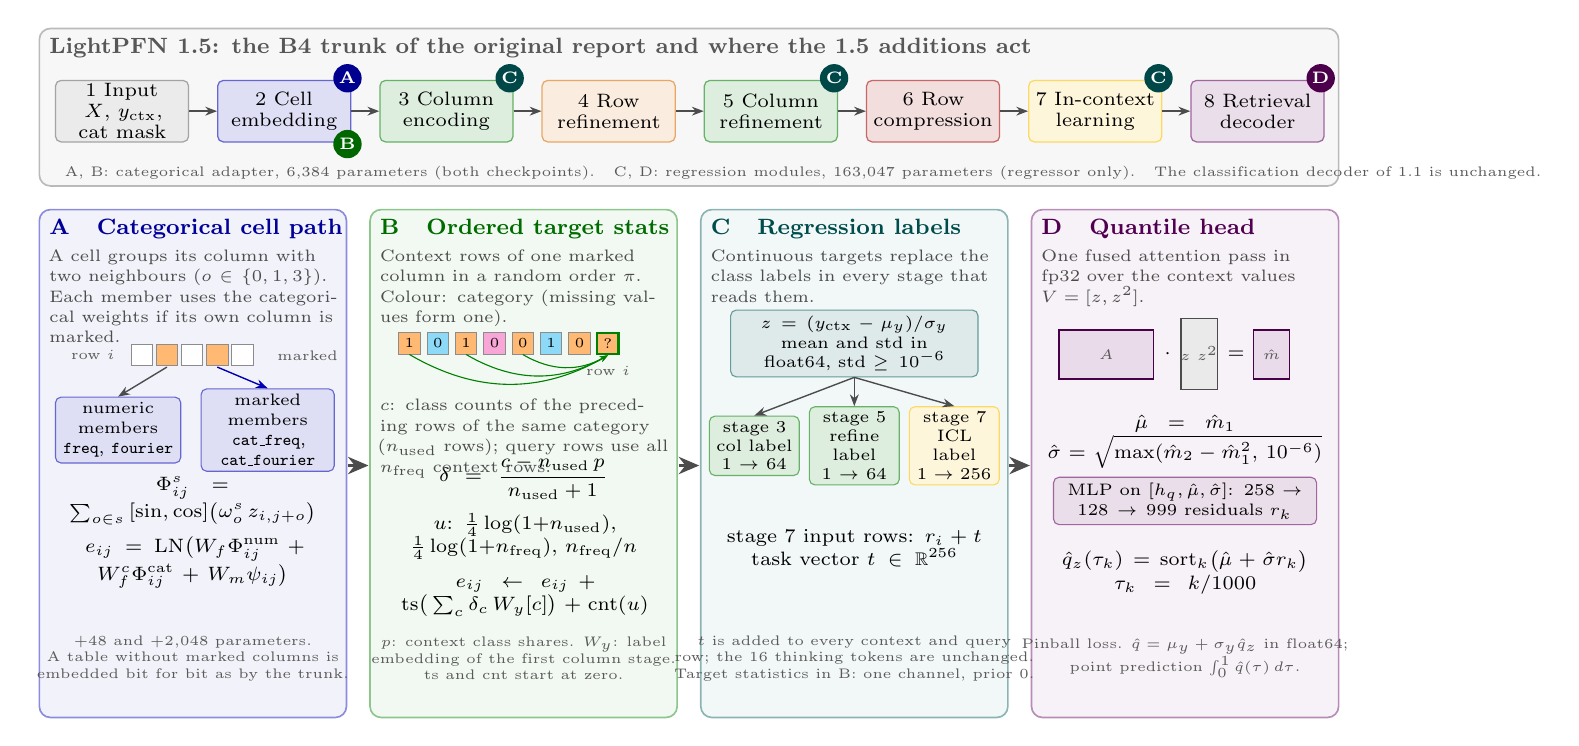
\begin{tikzpicture}[x=1cm, y=1cm]
\tikzset{eqs/.style={font=\fontsize{6.6}{8.4}\selectfont, align=center, inner sep=1pt, text width=3.7cm},
         txt/.style={font=\fontsize{6.2}{7.4}\selectfont, align=left, inner sep=0pt, text width=3.66cm, text=black!70},
         stage/.style={draw=#1!60, fill=#1!13, rounded corners=2pt, font=\fontsize{6.6}{7.6}\selectfont, align=center,
                       minimum height=0.78cm, text width=1.62cm, inner sep=1pt, line width=0.45pt},
         badge/.style={circle, fill=#1!80!black, text=white, font=\bfseries\fontsize{6.5}{7}\selectfont, inner sep=0.6pt,
                       minimum size=0.36cm},
         cat/.style={draw=black!45, line width=0.3pt, minimum width=0.27cm, minimum height=0.27cm, inner sep=0pt,
                     font=\fontsize{5.5}{6}\selectfont},
         mini/.style={draw=#1!60, fill=#1!13, rounded corners=2pt, font=\fontsize{6}{7.2}\selectfont, align=center,
                      inner sep=2pt, line width=0.4pt}}
\colorlet{cA}{blue!70!black}\colorlet{cB}{green!50!black}\colorlet{cC}{teal!70!black}\colorlet{cD}{violet!75!black}
\colorlet{k1}{orange!55}\colorlet{k2}{cyan!45}\colorlet{k3}{magenta!35}

% ---------------------------------------------------------------- trunk strip
\draw[panel=cin] (0,6.75) rectangle (16.5,8.75);
\node[stitle=cin] at (0.12,8.63) {LightPFN 1.5: the B4 trunk of the original report and where the 1.5 additions act};
\foreach \i/\c/\t in {0/cin/{1 Input\\$X$, $y_{\mathrm{ctx}}$, cat mask},
                      1/ccell/{2 Cell\\embedding},
                      2/ccol/{3 Column\\encoding},
                      3/cref/{4 Row\\refinement},
                      4/ccol/{5 Column\\refinement},
                      5/crow/{6 Row\\compression},
                      6/cicl/{7 In-context\\learning},
                      7/cdec/{8 Retrieval\\decoder}}
  \node[stage=\c] (s\i) at ({1.05+\i*2.06},7.7) {\t};
\foreach \i [evaluate=\i as \j using int(\i+1)] in {0,...,6} \draw[flow] (s\i.east) -- (s\j.west);
\node[badge=cA] at ($(s1.north east)+(-0.05,0.02)$) {A};
\node[badge=cB] at ($(s1.south east)+(-0.05,-0.02)$) {B};
\node[badge=cC] at ($(s2.north east)+(-0.05,0.02)$) {C};
\node[badge=cC] at ($(s4.north east)+(-0.05,0.02)$) {C};
\node[badge=cC] at ($(s6.north east)+(-0.05,0.02)$) {C};
\node[badge=cD] at ($(s7.north east)+(-0.05,0.02)$) {D};
\node[note, anchor=west] at (0.2,6.92) {A, B: categorical adapter, 6,384 parameters (both checkpoints).\quad
  C, D: regression modules, 163,047 parameters (regressor only).\quad The classification decoder of 1.1 is unchanged.};

% ---------------------------------------------------------------- panels
\def\W{3.9}\def\H{6.45}
\foreach \px/\c in {0/cA, 4.2/cB, 8.4/cC, 12.6/cD} \draw[panel=\c] (\px,0) rectangle ++(\W,\H);
\foreach \a in {3.9, 8.1, 12.3} \draw[bigflow] (\a+0.02,3.2) -- (\a+0.28,3.2);

% A: categorical cell path
\begin{scope}[shift={(0,0)}]
\node[stitle=cA] at (0.12,6.33) {A\quad Categorical cell path};
\node[txt, anchor=north west] at (0.12,5.95) {A cell groups its column with two neighbours ($o\in\{0,1,3\}$). Each member uses the categorical weights if its own column is marked.};
\foreach \j/\col in {0/white,1/k1,2/white,3/k1,4/white} \node[cat, fill=\col] at ({1.3+\j*0.32},4.6) {};
\node[note, anchor=east] at (1.08,4.6) {row $i$};
\node[note, anchor=west] at (2.9,4.6) {marked};
\node[mini=ccell, text width=1.45cm] (num) at (1.0,3.65) {numeric members\\\texttt{freq}, \texttt{fourier}};
\node[mini=cA, text width=1.55cm] (cat) at (2.9,3.65) {marked members\\\texttt{cat\_freq}, \texttt{cat\_fourier}};
\draw[flow] (1.62,4.45) -- (num.north); \draw[flow, cA] (2.26,4.45) -- (cat.north);
\node[eqs] at (1.95,2.35) {$\Phi^{s}_{ij}=\sum_{o\in s}\,[\sin,\cos]\big(\omega^{s}_o\,z_{i,j+o}\big)$\\[3pt]
  $e_{ij}=\mathrm{LN}\big(W_f\Phi^{\mathrm{num}}_{ij}+W^{c}_f\Phi^{\mathrm{cat}}_{ij}+W_m\psi_{ij}\big)$};
\node[note] at (1.95,0.75) {$+48$ and $+2{,}048$ parameters.\\A table without marked columns is\\embedded bit for bit as by the trunk.};
\end{scope}

% B: ordered target statistics
\begin{scope}[shift={(4.2,0)}]
\node[stitle=cB] at (0.12,6.33) {B\quad Ordered target stats};
\node[txt, anchor=north west] at (0.12,5.95) {Context rows of one marked column in a random order $\pi$. Colour: category (missing values form one).};
\foreach \j/\col/\y in {0/k1/1,1/k2/0,2/k1/1,3/k3/0,4/k1/0,5/k2/1,6/k1/0} \node[cat, fill=\col] (c\j) at ({0.5+\j*0.36},4.75) {\y};
\node[cat, fill=k1, line width=0.9pt, draw=cB] (ci) at ({0.5+7*0.36},4.75) {?};
\node[note] at ({0.5+7*0.36},4.4) {row $i$};
\foreach \j in {0,2,4} \draw[-{Stealth[length=1mm]}, cB, line width=0.4pt] (c\j.south) to[bend right=30] (ci.south);
\node[txt, anchor=north west] at (0.12,4.05) {$c$: class counts of the preceding rows of the same category ($n_{\mathrm{used}}$ rows); query rows use all $n_{\mathrm{freq}}$ context rows.};
\node[eqs] at (1.95,2.3) {$\delta=\dfrac{c-n_{\mathrm{used}}\,p}{n_{\mathrm{used}}+1}$\\[4pt]
  $u$: $\tfrac14\log(1{+}n_{\mathrm{used}})$, $\tfrac14\log(1{+}n_{\mathrm{freq}})$, $n_{\mathrm{freq}}/n$\\[4pt]
  $e_{ij}\leftarrow e_{ij}+\mathrm{ts}\big(\textstyle\sum_c\delta_c\,W_y[c]\big)+\mathrm{cnt}(u)$};
\node[note] at (1.95,0.75) {$p$: context class shares. $W_y$: label\\embedding of the first column stage.\\ts and cnt start at zero.};
\end{scope}

% C: regression labels
\begin{scope}[shift={(8.4,0)}]
\node[stitle=cC] at (0.12,6.33) {C\quad Regression labels};
\node[txt, anchor=north west] at (0.12,5.95) {Continuous targets replace the class labels in every stage that reads them.};
\node[mini=cC, text width=3.0cm] (z) at (1.95,4.75) {$z=(y_{\mathrm{ctx}}-\mu_y)/\sigma_y$\\mean and std in float64, std $\ge10^{-6}$};
\node[mini=ccol, text width=1.0cm, font=\fontsize{5.6}{6.8}\selectfont] (l3) at (0.68,3.45) {stage 3\\col label\\$1\to64$};
\node[mini=ccol, text width=1.0cm, font=\fontsize{5.6}{6.8}\selectfont] (l5) at (1.95,3.45) {stage 5\\refine label\\$1\to64$};
\node[mini=cicl, text width=1.0cm, font=\fontsize{5.6}{6.8}\selectfont] (l7) at (3.22,3.45) {stage 7\\ICL label\\$1\to256$};
\foreach \t in {l3,l5,l7} \draw[flow] (z.south) -- (\t.north);
\node[eqs] at (1.95,2.15) {stage 7 input rows: $r_i+t$\\task vector $t\in\mathbb{R}^{256}$};
\node[note] at (1.95,0.75) {$t$ is added to every context and query\\row; the 16 thinking tokens are unchanged.\\Target statistics in B: one channel, prior 0.};
\end{scope}

% D: moments and quantile head
\begin{scope}[shift={(12.6,0)}]
\node[stitle=cD] at (0.12,6.33) {D\quad Quantile head};
\node[txt, anchor=north west] at (0.12,5.95) {One fused attention pass in fp32 over the context values $V=[z,z^2]$.};
\matrixbox{0.35}{4.3}{1.2}{0.62}{cdec}
\node[note] at (0.95,4.61) {$A$};
\node[font=\scriptsize] at (1.73,4.61) {$\cdot$};
\matrixbox{1.9}{4.17}{0.46}{0.9}{cin}
\node[note] at (2.13,4.62) {$z\ z^2$};
\node[font=\scriptsize] at (2.6,4.61) {$=$};
\matrixbox{2.82}{4.3}{0.46}{0.62}{cdec}
\node[note] at (3.05,4.61) {$\hat m$};
\node[eqs] at (1.95,3.5) {$\hat\mu=\hat m_1$\\$\hat\sigma=\sqrt{\max(\hat m_2-\hat m_1^2,\,10^{-6})}$};
\node[mini=cD, text width=3.2cm] at (1.95,2.75) {MLP on $[h_q,\hat\mu,\hat\sigma]$: $258\to128\to999$ residuals $r_k$};
\node[eqs] at (1.95,1.85) {$\hat q_z(\tau_k)=\mathrm{sort}_k\big(\hat\mu+\hat\sigma r_k\big)$\\$\tau_k=k/1000$};
\node[note] at (1.95,0.75) {Pinball loss. $\hat q=\mu_y+\sigma_y\hat q_z$ in float64;\\point prediction $\int_0^1\hat q(\tau)\,d\tau$.};
\end{scope}
\end{tikzpicture}
}
\caption{LightPFN~1.5 architecture. Top: the eight operators of the B4 trunk of the original report, unchanged in 1.5, with the points where the additions act. \textbf{A}: categorical members of a cell group use their own Fourier frequencies and projection. \textbf{B}: ordered target statistics of each categorical cell, embedded through the label embedding of the first column stage and added to the cell embeddings. \textbf{C}: in the regressor, standardized targets replace the class-label embeddings in the column, column-refinement and ICL stages, and a task vector is added to every row entering the ICL stage. \textbf{D}: the retrieval decoder returns the first two moments of the context targets, from which a small MLP predicts 999 sorted quantiles. A table without categorical columns is processed exactly as by the trunk alone.}
\label{fig:arch2}
\end{figure}

\subsection{Categorical Adapter}
\label{sec:cat-adapter}

When \texttt{Config.cat\_adapter=True} is enabled, the model adds $6{,}384$ parameters ($4{,}609{,}472$ total for classification) split between the cell embedder and the first column stage (\texttt{lightpfn/model/lightpfn.py}, \texttt{lightpfn/model/catstats.py}): % runs/v15_5m_20261106/PROTOCOL.md
\begin{enumerate}
\item \textbf{Dedicated categorical Fourier embedding.}
In \texttt{CellEmbedder}, each cell groups its own column and two circular neighbors at offsets $o\in\{0,1,3\}$. Each member contributes its soft-clipped standardized value $z=5\tanh(((x-\mu)/(\sigma+10^{-6}))/5)$, expanded through 16 learned frequencies for that offset. The three sine/cosine vectors are summed before a shared bias-free projection $\R^{32}\to\R^{64}$. A separate projection embeds grouped standardized values, missingness flags, and rank Fourier features. % lightpfn/model/lightpfn.py:CellEmbedder
With \texttt{cat\_adapter=True}, a parallel set of learned frequencies \texttt{cat\_freq} ($3\times16=48$ parameters) and a bias-free projection \texttt{cat\_fourier} ($\R^{32}\to\R^{64}$, $2{,}048$ parameters) are added. % lightpfn/model/lightpfn.py
Group members with boolean categorical mask $\mathrm{cat}_j = 1$ route through \texttt{cat\_freq} and \texttt{cat\_fourier}, while columns with $\mathrm{cat}_j = 0$ use the numerical path.
\item \textbf{Ordered target statistics and count features.}
In \texttt{ColumnStage}, each categorical cell $(i,j)$ receives a vector of category statistics computed from the context rows $(X_{\text{ctx}}, y_{\text{ctx}})$. % lightpfn/model/catstats.py
Missing values (\texttt{NaN}) form a distinct category key of their own, and categories unseen in the context receive zero features.
For its category-specific counts, a context row $i$ excludes its own label: given a random permutation $\pi$ of the $n$ context rows, context row $i$ uses only the $n_{\text{used}}(i,j)$ context rows of the same category that precede it in $\pi$ (CatBoost's ordered target statistics \cite{prokhorenkova2018}). The global classification prior $p$ below still uses the full context class proportions.
Leave-one-out target statistics were tested during 1.1 development and caused a 12-point AUC collapse because leave-one-out statistics can encode a row's excluded label through category totals \cite[Section~12]{ottoboni2026lightpfn}. % docs/report/LightPFN_report.tex:Section12, runs/categorical/
Query rows $q$ use all $n_{\text{used}}(q,j) = n_{\text{freq}}(q,j)$ context rows belonging to their category, looked up via binary search against a per-category summary table cached during \texttt{encode}.

For a $C$-class classification task with empirical context class prior $p \in \R^C$ and smoothing parameter $\alpha = 1.0$ (\texttt{Config.cat\_smooth}), let $c(i,j) \in \R^C$ be the class counts among the $n_{\text{used}}(i,j)$ preceding context rows of cell $(i,j)$'s category, and let $n_{\text{freq}}(i,j)$ be the total number of other context rows in that category ($n_{\text{used}}$ for query rows).
The smoothed class-distribution deviation and the three count features are
\begin{equation}
\delta(i,j) = \frac{c(i,j) - n_{\text{used}}(i,j)\, p}{n_{\text{used}}(i,j) + \alpha}, \quad
u(i,j) = \left[ \tfrac{1}{4}\log(1 + n_{\text{used}}(i,j)),\, \tfrac{1}{4}\log(1 + n_{\text{freq}}(i,j)),\, \frac{n_{\text{freq}}(i,j)}{n} \right].
\label{eq:cat-stats}
\end{equation}
The module \texttt{CatStatsEmbed} maps $\delta(i,j)$ through the column stage label embeddings $W_y\in\R^{S\times64}$ and a learned bias-free matrix $\mathrm{ts}:\R^{64}\to\R^{64}$ ($4{,}096$ parameters), and maps $u(i,j)\in\R^3$ through a bias-free projection $\mathrm{cnt}:\R^3\to\R^{64}$ ($192$ parameters). Both projections start at zero. % lightpfn/model/lightpfn.py:CatStatsEmbed
At initialization (\texttt{cat\_freq} $=$ \texttt{freq}, \texttt{cat\_fourier} $=$ \texttt{fourier}, $\mathrm{ts}=0$, $\mathrm{cnt}=0$), the adapter initially reproduces the plain model up to floating-point rounding; when pretrained from scratch, all $6{,}384$ adapter parameters are learned jointly with the trunk.
\end{enumerate}

\subsection{Automatic Categorical Detection and Pretraining Mask-Drop}
\label{sec:cat-auto}

In scikit-learn workflows, users often pass NumPy arrays where categorical columns have already been ordinal-encoded as integers, without supplying a pandas \texttt{category} dtype or an explicit \texttt{cat} mask.
If a model is pretrained only with ground-truth masks, passing an unmasked integer-coded categorical column at test time routes it through the numerical cell path, which has never seen discrete category codes without adapter statistics.
We combine two mechanisms to handle this:
\begin{enumerate}
\item \textbf{Inference-time detection (\texttt{cat="auto"}).}
The helper \texttt{auto\_categorical(X)} (\texttt{lightpfn/sklearn.py}) marks any pandas \texttt{category}, string, object, or boolean column as categorical, and flags any numeric column whose non-missing training values are all exact integers with between 2 and 20 distinct values. % lightpfn/sklearn.py
On an 8,000-step V15 checkpoint, omitting the categorical mask (\texttt{cat=None} vs.\ ground-truth OpenML masks) costs $-0.21$ AUC points $[-0.43,-0.04]$ across D3 ($-0.63$ points on its 18 categorical tasks) and $-3.04$ points $[-5.83,-0.99]$ on Dcat 10k. % runs/analysis_cat_auto_20261105/RESULTS.md
Enabling \texttt{cat="auto"} reduces the gap to ground-truth masks to $-0.07$ points $[-0.21,+0.04]$ on D3 and $-0.39$ points $[-0.93,+0.08]$ on Dcat 10k; false positives on the 21 numerical D3 tasks with integer columns have a mean effect of $-0.008$ points. These are exploratory single-checkpoint measurements. % runs/analysis_cat_auto_20261105/RESULTS.md
\item \textbf{Pretraining categorical mask-drop (\texttt{--cat-mask-drop 0.25}).}
During classification pretraining, for each task independently, we clear its entire categorical mask with probability $p_{\text{drop}}=0.25$ before the forward pass. % lightpfn/train.py
This forces the numerical cell path and trunk to process categorical columns in 25\% of tasks (including high-cardinality columns with $>20$ levels that \texttt{cat="auto"} cannot distinguish from continuous integers) without adapter statistics.
In a 2,000-step A/B test, $p_{\text{drop}}=0.25$ shrinks the no-mask penalty (\texttt{none} minus \texttt{true}) from $-0.41$ to $-0.04$ points on D3 and from $-3.94$ to $-0.33$ points on Dcat 10k. % runs/analysis_cat_auto_20261105/RESULTS.md
In a paired 8,000-step confirmation, $p_{\text{drop}}=0.25$ vs.\ $p_{\text{drop}}=0$ shows no clear cost when the true mask is provided ($+0.03$ points on D1, $+0.05$ points $[-0.19, +0.27]$ on D3, and $-0.03$ points $[-0.46, +0.36]$ on Dcat 10k) while improving unmasked D3 AUC by $+0.34$ points $[-0.03, +0.77]$. % runs/analysis_cat_auto_20261105/RESULTS_md8k.md
\end{enumerate}

\subsection{Quantile Regression Head and Two-Member Wrapper}
\label{sec:reg-head}

To support regression without altering the classification trunk, \texttt{Config(head="quantiles")} adds a \texttt{RegressionModules} bundle of $163{,}047$ parameters (\texttt{lightpfn/model/regression.py}), bringing the regression checkpoint to $4{,}772{,}519$ parameters: % runs/v15_5m_20261106/PROTOCOL.md
\begin{enumerate}
\item \textbf{Target normalization and label embeddings.}
Given context targets $y_{\text{ctx}}\in\R^{B\times n}$, the model computes their mean $\mu_y$ and population standard deviation in \texttt{float64}, floors the standard deviation at $10^{-6}$, and returns standardized targets $z=(y_{\text{ctx}}-\mu_y)/\sigma_y$ in \texttt{float32}. % lightpfn/model/regression.py:normalize_targets
In the categorical adapter, ordered target statistics use a fixed zero prior ($\mu_z = 0$) and $C=1$ channel so a context row's own target never leaks through an empirical prior. % lightpfn/model/catstats.py
Continuous context targets are injected into the first column stage via \texttt{col\_label} ($\mathrm{Linear}(1, 64)$, 128 parameters), into the second column stage via \texttt{refine\_label} ($\mathrm{Linear}(1, 64)$, 128 parameters), and into the ICL stage via \texttt{icl\_label} ($\mathrm{Linear}(1, 256)$, 512 parameters), and a learned regression task token \texttt{task} $\in \R^{256}$ (256 parameters) is added to every context and query row at the input of the ICL stage (the 16 thinking tokens are unchanged). % lightpfn/model/regression.py
\item \textbf{Fused retrieval moments and 999-quantile residual head.}
At the end of the ICL stage, the retrieval decoder projects the normalized context representations to keys $K \in \R^{B \times H \times n \times d_h}$ ($H=4, d_h=16$) and the scaled query representations to queries $Q \in \R^{B \times H \times M \times d_h}$.
Rather than running two attention passes, \texttt{RetrievalDecoder.moments} concatenates $V = [z, z^2] \in \R^{B \times n \times 2}$ and executes a single fused scaled dot-product attention pass in \texttt{float32} to retrieve the local first and second moments $\hat{m}_1, \hat{m}_2 \in \R^{B \times M \times 1}$ averaged across the 4 heads: % lightpfn/model/lightpfn.py
\begin{equation}
\hat{\mu} = \hat{m}_1, \qquad \hat{\sigma} = \sqrt{\max\!\big(\hat{m}_2 - \hat{m}_1^2,\; 10^{-6}\big)}.
\label{eq:reg-moments}
\end{equation}
The \texttt{QuantileHead} ($162{,}023$ parameters: $\mathrm{Linear}(258, 128) \to \mathrm{GELU} \to \mathrm{Linear}(128, 999)$) takes $[h_{\text{query}}, \hat{\mu}, \hat{\sigma}] \in \R^{B \times M \times 258}$ and predicts $G=999$ raw scores $r \in \R^{B \times M \times 999}$ for the fixed quantile grid $\tau_k = k/1000$ ($k=1,\dots,999$).
The MLP outputs unconstrained residuals $r_k$. The model shifts and scales them by the retrieved moments, then sorts along the quantile axis:
\begin{equation}
\hat{q}_z(\tau_k) = \operatorname{sort}_{k}\!\left(\hat{\mu}+\hat{\sigma}r_k\right), \qquad k=1,\dots,999.
\label{eq:quantile-head}
\end{equation}
The output layer uses the standard linear-layer initialization; there is no softplus-increment parameterization or normal-quantile initialization. Predictions are unstandardized in \texttt{float64} via $\hat{q}(\tau_k)=\mu_y+\sigma_y\hat{q}_z(\tau_k)$.
Training minimizes mean pinball loss over the 999 levels in standardized units, approximating $\mathrm{CRPS}/(2\sigma_y)$. % lightpfn/model/regression.py
\item \textbf{Two-member inference wrapper.}
At inference (\texttt{V15Regressor} in \texttt{lightpfn/regressor.py}), the wrapper defaults to $n_{\text{estimators}}=2$ and $\text{max\_context}=50{,}000$.
The two members are encoded and queried in a single batched forward pass ($B=2$): member~1 fits the raw target $y$, while member~2 fits $\log(y)$ when $\min(y) > 0$ and the sample skewness of the context targets is at least 2 (the \texttt{log\_skew=2.0} default, Section~\ref{sec:reg-gap}; mapping predicted quantiles back via $\exp(\hat{q})$, clipped to the interval $[\max(2y_{\min}-y_{\max}, 0),$ $2y_{\max}-y_{\min}]$) or $-y$ otherwise (inverting and reversing the quantile grid via $-\hat{q}_{1-\tau}$).
The two monotone quantile curves are averaged ($L_2$ Wasserstein barycenter), and the point prediction for squared-error metrics (RMSE, $\mathrm{R}^2$) is the trapezoidal integral $\int_0^1 \hat{q}(\tau)\,d\tau = \E[Y \mid X]$ over $\tau_1,\dots,\tau_{999}$ with constant tail extrapolation on $[0, 0.001]$ and $[0.999, 1]$.
\end{enumerate}

% ======================================================================
\section{Prior and Data}
\label{sec:prior}

\subsection{Graph v4 vs.\ Graph v3 and the Class-Share Confound}
\label{sec:classeq}

In the 1.1 report, replacing the graph~v3 prior with graph~v4 (which reduces input outlier clipping and adds Zipf-quantized categorical columns up to 256 levels) appeared to hurt multiclass accuracy in short 500-step and 8,000-step tests \cite[Section~4]{ottoboni2026lightpfn}.
An audit of the generated task pools revealed a class-share confound: the graph~v3 generator used a binary-task probability of $p_{\mathrm{bin}}=0.55$ (leaving 45\% multiclass tasks with 3 to 10 classes), whereas the graph~v4 generator defaulted to $p_{\mathrm{bin}}=0.78$ (only 22\% multiclass tasks, or 27\% after mixing with rule tasks), while 28 of the 55 D3 tasks (51\%) are multiclass. % runs/v2_analysis_20261101/REPORT.md

To isolate the graph generator from the class distribution, we ran a controlled six-arm, 2,000-step experiment from random initialization (64 tasks/step, 90\% graph + 10\% rule) comparing $p_{\mathrm{bin}} \in \{0.55, 0.78\}$ and graph~v3 vs.\ graph~v4 on seed~0, with the $p_{\mathrm{bin}}=0.55$ graph comparison repeated on seed~1: % runs/v2_arch/classeq_v3v4_2k_20261101/RESULTS.md, DCAT_TAILS.md
\begin{itemize}
\item \textbf{Effect of $p_{\mathrm{bin}}$ within the same graph family.}
Raising $p_{\mathrm{bin}}$ from $0.55$ to $0.78$ degrades multiclass AUC in both priors: on D3 multiclass tasks, $p_{\mathrm{bin}}=0.78$ minus $0.55$ is $-0.61$ points raw ($-1.06$ EMA) for graph~v3 and $-1.26$ points raw ($-1.56$ EMA) for graph~v4, while binary D3 tasks are unchanged ($+0.14$ and $+0.11$ points raw, within noise). % runs/v2_arch/classeq_v3v4_2k_20261101/RESULTS.md
On D1 multiclass tasks, $p_{\mathrm{bin}}=0.78$ similarly loses $-0.49$ points raw ($-0.80$ EMA) for v3 and $-1.05$ points raw ($-1.28$ EMA) for v4. % runs/v2_arch/classeq_v3v4_2k_20261101/RESULTS.md
\item \textbf{Graph v4 vs.\ graph v3 at equal class share ($p_{\mathrm{bin}}=0.55$).}
When both generators use $p_{\mathrm{bin}}=0.55$, the multiclass gap vanishes: across seeds 0 and 1, graph~v4 minus graph~v3 is $+0.005$ and $+0.043$ points raw on D1, and $-0.041$ points $[-0.25,+0.19]$ and $-0.012$ points $[-0.24,+0.29]$ on D3. % runs/v2_arch/classeq_v3v4_2k_20261101/RESULTS.md
At the same time, on the 12 categorical cells of Dcat (6 datasets at 10,000 and 25,000 rows), graph~v4 at $p_{\mathrm{bin}}=0.55$ beats graph~v3 on both seeds: $+0.22$ points $[+0.10, +0.34]$ raw (10/12 cells; $+0.18$ EMA) on seed~0 and $+0.12$ points $[+0.004, +0.23]$ raw (9/12 cells; $+0.06$ EMA) on seed~1. % runs/v2_arch/classeq_v3v4_2k_20261101/DCAT_TAILS.md
\end{itemize}
LightPFN~1.5 classification pretraining therefore uses 90\% graph~v4 and 10\% rule~v1 with $p_{\mathrm{bin}}=0.55$ in both families. These are matched binary/multiclass task shares, not equal frequencies for all class counts.

\subsection{High-Cardinality Lookup Prior: Tried and Dropped}
\label{sec:lookup}

Because graph~v4 categorical columns are formed by Zipf-quantizing continuous latent variables (up to 256 levels), we tested whether adding a dedicated synthetic family of high-cardinality lookup tables (up to 1,000 levels with random per-level target effects, constrained to at least eight rows per level on average, \texttt{lightpfn/prior/lookup.py}) would further improve performance on high-cardinality categorical datasets.
In an 8,000-step $2\times 2$ factorial experiment comparing the plain B4 trunk against V15 ($\text{B4} + \text{categorical adapter}$), each trained on the same group-weighted mix (67.5\% short graph~v4, 22.5\% longer graph~v4, 10\% rule at $p_{\mathrm{bin}}=0.55$), with the lookup arms augmenting graph tasks with a lookup column at probability 20\%: % runs/v2_arch/lookup8k_20261104/COMPARE.md
\begin{itemize}
\item \textbf{Architectural effect (V15 minus B4 on the base prior, EMA 8k).}
Adding the categorical adapter improves D1, D3, Dcat, and the marked lookup probe; D2 falls from 0.9198 to 0.9173: D1 by $+0.31$ points $[+0.10, +0.53]$ (0.8569 vs.\ 0.8538), D3 by $+0.24$ points $[+0.01, +0.48]$ (0.8989 vs.\ 0.8965), Dcat 10k by $+2.30$ points (0.6939 vs.\ 0.6708, winning 5 of 6 datasets), Dcat 25k by $+2.12$ points (0.6982 vs.\ 0.6770, 5 of 6), and the synthetic high-cardinality lookup probe by $+9.28$ points averaged over cardinalities ($K=1024$: 0.7115 vs.\ 0.6588, a $+5.27$-point gain). % runs/v2_arch/lookup8k_20261104/COMPARE.md
\item \textbf{Prior effect (V15 with lookup prior minus V15 on base prior, EMA 8k).}
Adding the lookup prior degrades D1 by $-0.48$ points $[-0.68, -0.29]$ (0.8521 vs.\ 0.8569) and D3 by $-0.17$ points $[-0.37, +0.06]$ (0.8972 vs.\ 0.8989), fails to improve Dcat ($-0.27$ points at 10k, 0.6912 vs.\ 0.6939; $-0.10$ points at 25k, 0.6972 vs.\ 0.6982), and adds only $+0.92$ points on the lookup probe itself. % runs/v2_arch/lookup8k_20261104/COMPARE.md
\end{itemize}
The categorical adapter already learns to exploit per-level target statistics from the Zipf-quantized categorical columns of graph~v4; adding these lookup columns reduced D1 accuracy without improving Dcat in this one-seed test, so we dropped the lookup prior.

\subsection{Regression Prior \texttt{r2} and Learnability Audit}
\label{sec:r2-prior}

Our initial synthetic regression generator (P0, \texttt{lightpfn/prior/regression.py} and \texttt{observation.py}) extracted a continuous target node from the SCM, standardized its location on 2,048 disjoint calibration rows, and passed it through one of nine observation channels (Gaussian, heteroscedastic Gaussian, Student-$t$, sinh-arcsinh, positive log-location, bimodal mixture, zero-inflated hurdle, Poisson-gamma counts, or top-coded censoring).
Auditing 1,024 P0 tasks against the 23 real OpenML regression datasets of D3-reg exposed three mismatches: % runs/analysis_reg_prior_20261104/SUMMARY.md
(1) \emph{unlearnable tasks:} on 36.3\% of P0 tasks, a 200-tree ExtraTrees regressor with \texttt{min\_samples\_leaf=2} achieved held-out $\mathrm{R}^2 \le 0$ on a 70/30 split (median $\mathrm{R}^2 = 0.145$), vs.\ only 4.3\% (1 of 23 tasks) on D3-reg (median $\mathrm{R}^2 = 0.776$); % runs/analysis_reg_prior_20261104/SUMMARY.md
(2) \emph{excessive channel noise and weak nonlinear signal:} only 15.5\% of P0 tasks had $\mathrm{R}^2_{\text{ET}} - \mathrm{R}^2_{\text{Ridge}} > 0.10$, vs.\ 34.8\% on D3-reg; % runs/analysis_reg_prior_20261104/SUMMARY.md
and (3) \emph{lack of discrete/rounded targets and heavy tails:} 43.5\% of D3-reg datasets have unique-value ratio $< 0.5$ vs.\ 6.6\% in P0, and 90th-percentile target skewness ($4.51$ vs.\ $2.80$) and excess kurtosis ($43.49$ vs.\ $18.13$) were higher in real data. % runs/analysis_reg_prior_20261104/SUMMARY.md

We addressed these in the \texttt{r2} regression prior recipe (\texttt{--reg-factors} set to \texttt{filter}, \texttt{noise}, \texttt{tails}, \texttt{discrete}): % lightpfn/prior/regression.py, lightpfn/prior/observation.py
\begin{itemize}
\item \texttt{filter}: fits a 32-tree ExtraTrees regressor on the 2,048 independent calibration rows to predict the latent SCM location from the features, and rejects structural drafts with OOB $\mathrm{R}^2<0.10$ while retaining 5\% of failing drafts. Observed noisy targets are not used in this filter. % lightpfn/prior/regression.py:SIGNAL_FILTER
\item \texttt{noise} and \texttt{tails}: tightens additive noise to $[0.02, 1.0]$ and log-scale noise to $[0.03, 0.70]$, links hurdle zero probabilities to the latent location via a logistic link, reduces the bimodal gap parameter to $[0.3,1.5]$, widens positive log-spread to $[0.3, 1.5]$, and upweights skewed/count/censored channels.
\item \texttt{discrete}: with probability $0.35$ on eligible continuous channels, rounds targets to a grid whose step is sampled log-uniformly from $[0.05,1.0]$ times a declared channel-dependent unit. % lightpfn/prior/observation.py:RANGES_R2,grid_unit
\end{itemize}
In 2,000-step A/B tests across two seeds, \texttt{r2} on graph~v3 lowered D3-reg raw normalized CRPS by $-4.7\%$ $[-7.5\%, -2.5\%]$ on seed~0 (19/23 tasks) and $-3.4\%$ $[-6.9\%, -1.1\%]$ on seed~1 (19/23 tasks), for a two-seed mean reduction of $-4.1\%$ $[-7.0\%, -1.9\%]$ (21/23 tasks), outperforming \texttt{r2} on graph~v4 ($-3.3\%$ mean across seeds). % runs/analysis_reg_prior_20261105/AB_RESULTS_s1.md
We therefore selected \texttt{r2} on graph~v3 for regression pretraining (noting in Section~\ref{sec:reg-gap} a subtle interaction with categorical cardinality in graph~v3 uncovered after training).

% ======================================================================
\section{Negative Result: The Candidate ``v2'' Architecture (A3)}
\label{sec:negative}

Before adopting the B4-based LightPFN~1.5 design, we investigated a redesigned 4.8-million-parameter candidate trunk, denoted A3 (or C2v2), which used 8 distinct (unshared) ICL blocks with a reduced MLP ratio to stay under 5 million parameters, a heavier cell frontend with an explicit level-ID embedding view, and an unshared retrieval decoder. % docs/v2.md, runs/v2_arch/box_20261031/RESULTS.md

\paragraph{Late training instability and decoder diagnostics.}
While A3 performed well in 8,000-step screens, it became unstable in 30,000-step pretraining runs: at peak learning rate $5\cdot 10^{-4}$ it diverged between 9,500 and 15,000 steps, and at $10^{-3}$ it completed 30,000 steps but fell far behind the v1 30,000-step checkpoint (D1 $-2.83$ points, D2 $-5.20$ points, D3 $-0.95$ points). % runs/v2_arch/instability_20261031/EVIDENCE.md, runs/v2_arch/instability_review_20261103/REPORT.md
A replay of nine checkpoints across 1,728 forward/backward replays documented two growing decoder scale components in the retrieval decoder: % runs/v2_arch/instability_review_20261103/REPORT.md
(1) in \texttt{SoftmaxScaling}, the effective scaling base at context length $n=1024$ grew from $10.9$ at 7,500 steps to $1{,}246$ at 30,000 steps (vs.\ $1.6$ in v1), while the participation ratio of the 64-dimensional diagonal query/key metric collapsed from 42 dimensions to 5; % runs/v2_arch/instability_review_20261103/REPORT.md
and (2) in the original unbounded run, the product of the learned RMSNorm affine gains on the retrieval queries and keys grew from $1.05$ to $7.93$. % runs/v2_arch/instability_20261031/QK_GAINS.md
Post-hoc interventions on the damaged 30,000-step checkpoint (temperature clipping, FP64 decoding, or removing affine gains at inference) could not recover v1 accuracy, consistent with coadaptation of the decoder and upstream representations; the replay does not establish the original cause. % runs/v2_arch/instability_review_20261103/REPORT.md

\paragraph{Stabilized 30,000-step paired gate.}
Setting \texttt{decoder\_scale\_mode="atan"} and removing the retrieval query/key affine weights (\texttt{Config.retrieval\_qk\_affine=False}, bounding retrieval logits by $|\text{logit}| \le 64$ by construction) produced a stable 30,000-step run; it does not establish stability beyond that budget.
In a pre-declared, paired 30,000-step gate comparing B4 against stabilized A3 on the exact same data stream (64 tasks/step, graph~v4 + rule at $p_{\mathrm{bin}}=0.55$), A3 trained with zero non-finite gradients for all 30,000 steps, but failed the quality gate against B4 on EMA weights: D3 AUC was $-0.14$ points $[-0.26, -0.03]$ (0.9043 vs.\ 0.9057), D1 was $-0.54$ points $[-0.77, -0.32]$ (0.8664 vs.\ 0.8718, losing $-1.94$ points on rule tasks), D2 was $-1.21$ points (0.9235 vs.\ 0.9356), and CPU inference at 100 columns was $1.6\text{--}1.7\times$ slower than B4. % runs/v2_arch/v1v2_30k_20261104/RESULTS.md, runs/v2_arch/instability_review_20261103/REPORT.md
Meanwhile, B4 with the 6,384-parameter categorical adapter at 8,000 steps already exceeded A3's 30,000-step Dcat 10k score (0.6939 vs.\ 0.6864). % runs/v2_arch/lookup8k_20261104/COMPARE.md
We therefore abandoned A3 and built LightPFN~1.5 on the B4 trunk.

% ======================================================================
\section{Training Recipe and Selection Protocol}
\label{sec:training}

\subsection{Training Stages}
\label{sec:schedule}

\begin{figure}[tbp]
\centering
\resizebox{\linewidth}{!}{% LightPFN 1.5 training pipeline: five stages and the gates. Sources: runs/v15_5m_20261106/PROTOCOL.md,
% runs/remote/stage2_box_20261108/HANDOFF.md, runs/cls_wide_20261109/PROTOCOL.md, runs/reg_wide_20261109/RESULTS.md.
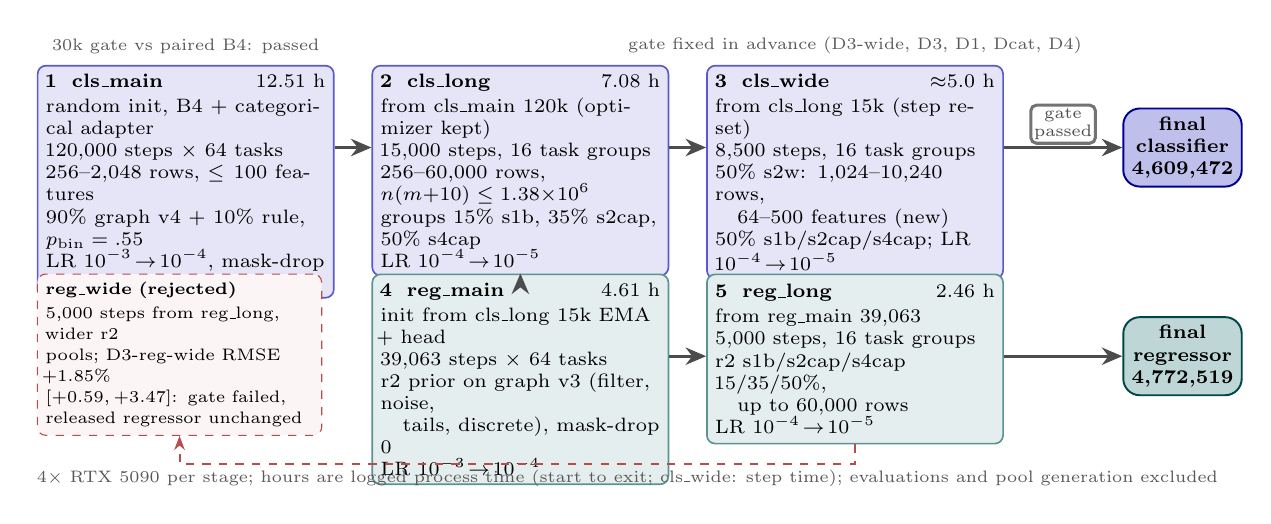
\begin{tikzpicture}[x=1cm, y=1cm]
\tikzset{
  st/.style={draw=#1!65, fill=#1!10, rounded corners=3pt, line width=0.6pt, align=left, inner sep=3pt,
             text width=3.55cm, font=\fontsize{6.6}{8}\selectfont, minimum height=2.15cm, anchor=north west},
  ckpt/.style={draw=#1!80!black, fill=#1!25, rounded corners=6pt, font=\bfseries\fontsize{6.8}{8}\selectfont,
               align=center, inner sep=3pt, line width=0.7pt},
  gate/.style={draw=black!55, fill=white, rounded corners=2pt, inner sep=1.2pt, font=\fontsize{5.8}{6.5}\selectfont,
               align=center},
  lab/.style={font=\fontsize{6}{7}\selectfont, text=black!65, align=center},
}
\colorlet{ccls}{blue!70!black}\colorlet{creg}{teal!70!black}\colorlet{cfail}{red!60!black}

\node[st=ccls] (main) at (0,4.6) {\textbf{1\ \ cls\_main} \hfill 12.51 h\\[1pt]
  random init, B4 $+$ categorical adapter\\120,000 steps $\times$ 64 tasks\\
  256--2,048 rows, $\le100$ features\\90\% graph v4 $+$ 10\% rule, $p_{\mathrm{bin}}=.55$\\
  LR $10^{-3}\!\to\!10^{-4}$, mask-drop .25};
\node[st=ccls] (long) at (4.25,4.6) {\textbf{2\ \ cls\_long} \hfill 7.08 h\\[1pt]
  from cls\_main 120k (optimizer kept)\\15,000 steps, 16 task groups\\
  256--60,000 rows, $n(m{+}10)\le1.38{\times}10^6$\\groups 15\% s1b, 35\% s2cap, 50\% s4cap\\
  LR $10^{-4}\!\to\!10^{-5}$};
\node[st=ccls] (wide) at (8.5,4.6) {\textbf{3\ \ cls\_wide} \hfill $\approx$5.0 h\\[1pt]
  from cls\_long 15k (step reset)\\8,500 steps, 16 task groups\\
  50\% s2w: 1,024--10,240 rows,\\\quad 64--500 features (new)\\
  50\% s1b/s2cap/s4cap; LR $10^{-4}\!\to\!10^{-5}$};
\node[ckpt=ccls] (fc) at (14.55,3.55) {final\\classifier\\4,609,472};

\node[st=creg] (rmain) at (4.25,1.95) {\textbf{4\ \ reg\_main} \hfill 4.61 h\\[1pt]
  init from cls\_long 15k EMA $+$ head\\39,063 steps $\times$ 64 tasks\\
  r2 prior on graph v3 (filter, noise,\\\quad tails, discrete), mask-drop 0\\
  LR $10^{-3}\!\to\!10^{-4}$};
\node[st=creg] (rlong) at (8.5,1.95) {\textbf{5\ \ reg\_long} \hfill 2.46 h\\[1pt]
  from reg\_main 39,063\\5,000 steps, 16 task groups\\
  r2 s1b/s2cap/s4cap 15/35/50\%,\\\quad up to 60,000 rows\\
  LR $10^{-4}\!\to\!10^{-5}$};
\node[ckpt=creg] (fr) at (14.55,0.9) {final\\regressor\\4,772,519};

\draw[bigflow] (main.east |- 0,3.55) -- (long.west |- 0,3.55);
\draw[bigflow] (long.east |- 0,3.55) -- (wide.west |- 0,3.55);
\draw[bigflow] (wide.east |- 0,3.55) -- node[gate, above=1pt] {gate\\passed} (fc.west);
\draw[bigflow] ($(long.south)+(0,0)$) -- (rmain.north);
\draw[bigflow] (rmain.east |- 0,0.9) -- (rlong.west |- 0,0.9);
\draw[bigflow] (rlong.east |- 0,0.9) -- (fr.west);
\node[lab, anchor=south] at ($(main.north)+(0,0.02)$) {30k gate vs paired B4: passed};
\node[lab, anchor=south] at ($(wide.north)+(0,0.02)$) {gate fixed in advance (D3-wide, D3, D1, Dcat, D4)};

% rejected regression wide fine-tune
\node[draw=cfail!70, dashed, rounded corners=3pt, fill=cfail!4, font=\fontsize{6.4}{7.6}\selectfont, align=left,
      text width=3.4cm, anchor=north west, inner sep=3pt] (rw) at (0,1.95) {\textbf{reg\_wide (rejected)}\\[1pt]
  5,000 steps from reg\_long, wider r2\\pools; D3-reg-wide RMSE $+1.85\%$\\$[+0.59,+3.47]$: gate failed,\\released regressor unchanged};
\draw[-{Stealth[length=1.8mm]}, cfail!70, dashed, line width=0.7pt] (rlong.south) -- ++(0,-0.25) -| (rw.south);
\node[lab, anchor=north] at (7.5,-0.42) {4$\times$ RTX 5090 per stage; hours are logged process time (start to exit; cls\_wide: step time); evaluations and pool generation excluded};
\end{tikzpicture}
}
\caption{Training pipeline of LightPFN~1.5. Each box gives the initialization, steps, data and learning-rate schedule of one stage, with the logged hours on 4$\times$ RTX~5090. The final classifier comes from the wide-table fine-tuning, which passed a gate declared before its evaluation; the final regressor is the end of the long-context regression stage. A wide-table regression fine-tuning (dashed) failed its gate and was not released (Section~\ref{sec:reg-wide}).}
\label{fig:stages}
\end{figure}

LightPFN~1.5 is trained in five stages (Figure~\ref{fig:stages}): three for the classifier (main pretraining, long-context training and a wide-table fine-tuning) and two regression fine-tuning stages starting from the long-context classifier, all using data-parallel training across four NVIDIA RTX~5090 GPUs per stage with \texttt{bfloat16} mixed precision, Muon \cite{jordan2024muon} for internal block matrices, AdamW ($\beta_1=0.9, \beta_2=0.98$, weight decay $0.01$) for the remaining parameters, gradient clipping at $1.0$, and EMA decay $0.999$: % runs/v15_5m_20261106/PROTOCOL.md, recipe.py
\begin{enumerate}
\item \textbf{Main classification stage (\texttt{cls\_main}, 120,000 steps).}
Initialized from random weights with $\text{B4} + \texttt{cat\_adapter=True}$ ($4{,}609{,}472$ parameters).
Trains for 120,000 steps at 64 tasks per step ($7{,}680{,}000$ task draws across 16 streamed pool pairs of 252,160 generated tasks each, $4.03\times 10^6$ unique tasks, a two-pass sizing budget with a 5\% generation margin) on 90\% graph~v4 + 10\% rule~v1 ($p_{\mathrm{bin}}=0.55$, 256--2,048 rows, $\le 100$ features, $\texttt{--cat-mask-drop 0.25}$, warmup 2,000, cosine LR $10^{-3}\to 10^{-4}$, $800{,}000$ cells/GPU). % runs/v15_5m_20261106/PROTOCOL.md
\item \textbf{Long-context classification stage (\texttt{cls\_long}, 15,000 steps).}
Resumes from \texttt{cls\_main} step 120,000 (warmup 200, cosine LR $10^{-4}\to 10^{-5}$, $\texttt{--cat-mask-drop 0.25}$).
Each step draws 16 task groups across the 4 GPUs (an expected $57.6$ tasks/step and $864{,}000$ task draws) from three row-count regimes (90\% graph~v4 + 10\% rule at $p_{\mathrm{bin}}=0.55$):
15\% from \texttt{s1b} (256--2,048 rows, 8 tasks/group),
35\% from \texttt{s2cap} (1,024--10,240 rows, 4 tasks/group, with the preset feature cap), and
50\% from \texttt{s4cap} (4,096--60,000 rows, 2 tasks/group, capped at $800{,}000$ cells). % runs/v15_5m_20261106/PROTOCOL.md
Micro-batches enforce $n(m+10)\le1.38\times10^6$ with \texttt{--fit-rows}. These row-count ranges refer to the whole synthetic table, including context and query rows.
The 15,000-step EMA checkpoint (\texttt{cls\_long/ema\_step015000.pt}) initializes the regression stages and the wide-table fine-tuning below.
\item \textbf{Main regression fine-tuning stage (\texttt{reg\_main}, 39,063 steps).}
Two pilot tests guided this stage: first, in a 2,000-step, two-seed pilot comparing the 999-grid \texttt{quantiles} head against a distributional \texttt{transport} head, \texttt{transport} had $+18.0\%$ $[+7.5\%, +31.8\%]$ worse normalized CRPS on D3-reg, so \texttt{quantiles} was chosen; % runs/v2_arch/reg_heads_20261104/TABLES.md
second, warm-starting V15 regression from a pretrained classification checkpoint reduced 2,000-step D3-reg CRPS by $-10.1\%$ raw ($-15.5\%$ EMA: 0.2122 vs.\ 0.2490) relative to training from scratch, matching 18,000 steps of scratch training in 2,000 steps and reaching 0.1975 EMA CRPS at 10,000 steps. % runs/analysis_reg_v15_20261105/RESULTS_s0.md
We therefore initialize \texttt{reg\_main} from the final \texttt{cls\_long} EMA checkpoint (\texttt{--init}) and fine-tune the network with $4{,}772{,}519$ stored parameters for $39{,}063$ steps $\times 64$ tasks/step $= 2{,}500{,}032$ task draws (13 streamed pools of $105{,}216$ \texttt{r2} graph~v3 tasks each, $1.37\times 10^6$ unique tasks, warmup 200, cosine LR $10^{-3}\to 10^{-4}$, $400{,}000$ cells/GPU, $\texttt{--cat-mask-drop 0}$). % runs/remote/stage2_box_20261108/HANDOFF.md
\item \textbf{Long-context regression stage (\texttt{reg\_long}, 5,000 steps).}
Resumes from \texttt{reg\_main} step 39,063 for 5,000 steps (warmup 200, cosine LR $10^{-4}\to 10^{-5}$, 16 groups/step, an expected $288{,}000$ task draws across 15\% \texttt{r2\_s1b}, 35\% \texttt{r2\_s2cap}, and 50\% \texttt{r2\_s4cap}, $n(m+10)\le 1.38\times 10^6$ with \texttt{--fit-rows}). % runs/remote/stage2_box_20261108/HANDOFF.md
Both regression stages enable \texttt{LIGHTPFN\_NAN\_GUARD}, which captures diagnostics and aborts before an update on non-finite gradients or a non-finite gradient norm; it does not zero gradients or skip bad updates silently. All $44{,}063$ production regression steps completed without a recorded guard failure. An earlier short pilot had a non-finite-gradient failure that was not reproduced in the subsequent diagnostic replays. % lightpfn/train.py:NanGuard, runs/v15_5m_20261106/NAN_GUARD.md, runs/remote/stage2_box_20261108/REGDIAG.md
The 5,000-step EMA checkpoint (\texttt{reg\_long/ema\_step005000.pt}) is the final LightPFN~1.5 regressor.
\end{enumerate}

\paragraph{Wide-table classification fine-tuning (\texttt{cls\_wide}, 8,500 steps).}
Pretraining never generated more than 100 features, and a comparison of 1.5 with 1.1.0 found one repeated weakness: tables with more than 60 to 100 features. % runs/analysis_cls_v2gap_20261109/RESULTS.md
We therefore continue the \texttt{cls\_long} checkpoint (model, EMA and optimizer state, step counter reset) for 8,500 steps with the same optimizer settings (warmup 200, cosine LR $10^{-4}\to 10^{-5}$, $\texttt{--cat-mask-drop 0.25}$, $n(m+10)\le1.38\times10^6$) and fresh pools of the same generators: 8\% \texttt{s1b}, 17\% \texttt{s2cap}, 25\% \texttt{s4cap}, and 50\% \texttt{s2w}, a new pool with 1,024--10,240 rows and 64--500 features (at most $10^6$ cells). The step count was fixed from the measured step time before any quality result, and the gate was declared in advance: on the final EMA only, D3-wide (the nine D3 datasets with more than 100 features, all columns) must improve in AUC or log loss with the 95\% interval excluding zero, D3 must not lose more than 0.10 points, and D1, Dcat and D4 must not worsen beyond noise; only then is TabArena-Lite run. % runs/cls_wide_20261109/PROTOCOL.md
The final EMA (\texttt{cls\_wide/ema\_step008500.pt}, about 5.0~h of logged step time on 4$\times$ RTX~5090) passes the gate and is the final LightPFN~1.5 classifier (Section~\ref{sec:cls-wide}).

\paragraph{Compute budget.}
Each stage used a node with 4$\times$ NVIDIA RTX~5090 GPUs (32~GiB VRAM each) and an AMD EPYC~9654 CPU. Main classification and the remaining stages ran on two successive rented nodes; CPU pool generation overlapped training. % runs/v15_5m_20261106/BOX_4GPU.md, runs/remote/stage2_box_20261108/HANDOFF.md
Summing the logged start-to-exit intervals of the training processes gives $12.51$~h for \texttt{cls\_main}, $7.08$~h for \texttt{cls\_long}, $4.61$~h for \texttt{reg\_main}, and $2.46$~h for \texttt{reg\_long}: $26.7$~h. The wide-table fine-tuning was paused twice for milestone evaluations; the sum of its logged step times is $5.01$~h. In total, approximately \textbf{31.7 hours} or \textbf{127 RTX~5090 GPU-hours}. These intervals include process startup and saving (except for \texttt{cls\_wide}), but exclude separate evaluations, pool generation, pilots, the rejected regression fine-tuning, and earlier model-development experiments. They are not the total project compute budget. % runs/cls_wide_20261109/box/train/log.csv % runs/remote/stage2_box_20261108/copy_59705041/LightPFN/runs/v15_5m_20261106/out/events.log

\subsection{Selection Protocol}
\label{sec:protocol}

Following \cite[Section~3]{ottoboni2026lightpfn}, all architectural, prior, and hyperparameter decisions were made on datasets disjoint from TabArena \cite{tabarena}:
\textbf{D1} (1,536 held-out synthetic classification tasks: 384 each from graph~v3, graph~v4, rule~v1, and tree~v4);
\textbf{D2} (125 synthetic mechanism probes);
\textbf{D3} (the 55 OpenML-CC18 classification datasets outside TabArena, 5-fold stratified CV at $\le 1{,}000$ rows, $\le 100$ features);
\textbf{Dcat} (6 large OpenML categorical datasets outside TabArena and D3 with $>2$ category levels: \emph{albert}, \emph{porto-seguro}, \emph{kick}, \emph{okcupid-stem}, \emph{sf-police-incidents}, \emph{airlines}, evaluated at 10,000 and 25,000 training rows with 1 estimator and full context); % runs/catft/dcat.py
\textbf{Scale} (15 datasets, 162 splits from 1k to 94,320 training rows) and \textbf{D4} (13 large datasets, 46 splits at 10k--100k rows);
and for regression, \textbf{D1-reg} (36 synthetic tasks), \textbf{D3-reg} (23 OpenML-CTR23 regression datasets outside TabArena, 115 five-fold splits at $\le 1{,}000$ rows), and \textbf{D3-reg-L} (the 15 D3-reg datasets with $\ge 4{,}000$ finite rows, 30 splits up to 40,000 training rows). % lightpfn/eval/external_reg.py, runs/analysis_reg_inference_20261109/RESULTS.md
TabArena was reserved for final evaluation, with one exception: during the wide-table fine-tuning (Section~\ref{sec:cls-wide}) the first TabArena split, scored from saved predictions, entered the pre-declared early-stop and extension rules (not the gate), so it is not an independent test of that stage.

% ======================================================================
\section{Results: Classification}
\label{sec:cls-results}

\subsection{Milestone Progression and External Benchmarks (D1, D2, D3, Dcat, Scale, D4)}
\label{sec:cls-milestones}

Table~\ref{tab:milestones} tracks the EMA checkpoints of LightPFN~1.5 across \texttt{cls\_main} (30k, 60k, 90k, 120k steps) and \texttt{cls\_long} (+5k, +10k, +15k steps, up to 135k total) alongside LightPFN~1.0 (30k and the released 120k), LightPFN~1.1.0 (\texttt{final\_long}, 159.25k total steps), and default GBDT baselines ($n_{\text{estimators}}=1$, ground-truth dataset categorical masks).
Figure~\ref{fig:cls} plots the progression on D1, D3 and Dcat 10k across the schedule and the per-dataset Dcat breakdown against larger foundation models.

\begin{table}[tbp]
\centering
\footnotesize
\setlength{\tabcolsep}{3.8pt}
% Classification milestone table: D1, D2, D3, Dcat 10k, Dcat 25k, Scale, and D4.
% Source files: plotdata2/cls_milestones.dat, plotdata2/dcat_tasks.dat, runs/v15_5m_20261106/out/eval/*.json,
% runs/dev/final*, runs/eval/external/*.csv, runs/catft/dcat/*.csv, runs/eval/large/*.csv, runs/eval/scale/*.csv.
\begin{tabular}{llcccccccc}
\toprule
Model / stage & steps & D1 & D2 & D3 AUC & D3 log loss & Dcat 10k & Dcat 25k & Scale & D4 \\
\midrule
% runs/eval/external/{catboost,lightgbm,xgboost}.csv, runs/eval/large/{catboost,lightgbm,xgboost}.csv, runs/eval/scale/catboost.csv
CatBoost (default) & -- & -- & -- & .9023 & .4012 & .7031 & .7118 & .9071 & .8189 \\
LightGBM (default) & -- & -- & -- & .8907 & .5174 & .6809 & .6829 & -- & .7848 \\
XGBoost (D3: 54 tasks) & -- & -- & -- & .8889 & .5213 & .6421 & .6597 & -- & .7903 \\
\midrule
% runs/dev/final_s30000/*, runs/eval/external/final_s30000_n1.csv, runs/catft/dcat/final_s30000.csv
LightPFN 1.0 (v1 30k) & 30k & .8703 & .9373 & .9054 & .3807 & .6706 & .6733 & -- & -- \\
% runs/dev/final/*, runs/eval/external/final_n1.csv, runs/eval/large/final_full.csv
LightPFN 1.0 (\texttt{final}) & 120k & .8781 & .9331 & .9104 & .3586 & .6895 & .6935 & .9025 & .8063 \\
% runs/dev/final_long_s39250/*, runs/eval/external/final_long_s39250_n1.csv, runs/catft/dcat/plain.csv, runs/eval/large/final_long_s39250_full.csv
LightPFN 1.1.0 (\texttt{final\_long}) & 159.25k & .8783 & .9391 & .9109 & .3550 & .7047 & .7098 & .9097 & .8188 \\
\midrule
% runs/v15_5m_20261106/out/eval/v15_5m_20261106_cls_main_ema_s{030000,060000,090000,120000}.json
1.5 \texttt{cls\_main} & 30k & .8713 & .9359 & .9054 & .3763 & .6703 & -- & -- & -- \\
1.5 \texttt{cls\_main} & 60k & .8744 & .9444 & .9074 & .3677 & .6766 & -- & -- & -- \\
1.5 \texttt{cls\_main} & 90k & .8775 & .9392 & .9098 & .3610 & .7025 & -- & -- & -- \\
1.5 \texttt{cls\_main} & 120k & .8779 & .9485 & .9094 & .3594 & .7016 & -- & -- & -- \\
% runs/v15_5m_20261106/out/eval/v15_5m_20261106_cls_long_ema_s{005000,010000,015000}*
1.5 \texttt{cls\_long} (+5k) & 125k & .8772 & .9481 & .9103 & .3586 & .7078 & -- & -- & -- \\
1.5 \texttt{cls\_long} (+10k) & 130k & .8774 & .9474 & .9104 & .3583 & .7056 & -- & -- & -- \\
\rowcolor{orange!12}
1.5 \texttt{cls\_long} (+15k, final) & 135k & .8777 & .9531 & .9103 & .3582 & .7075 & .7134 & .9102 & .8200 \\
\bottomrule
\end{tabular}

\caption{Classification benchmark progression across training milestones (mean ROC AUC, and mean log loss on D3; single estimator, full context). D1: 1,536 held-out synthetic tasks; D2: 125 mechanism probes; D3: 55 OpenML-CC18 tasks outside TabArena; Dcat 10k / 25k: 6 high-cardinality categorical datasets at 10,000 and 25,000 training rows; Scale: 162 splits across 15 datasets (1k--94,320 training rows); D4: 46 splits across 13 large datasets (10k--100k rows). The released LightPFN~1.0 row uses the 120k-step checkpoint on all suites. XGBoost D3 excludes its failed task (54 tasks); the other D3 entries use 55.}
\label{tab:milestones}
\end{table}

\begin{figure}[tbp]
\centering
\resizebox{\linewidth}{!}{% Classification progression of the 1.5 schedule (top: D1, D3, Dcat 10k vs training step, single estimator) and
% per-dataset Dcat 10k AUC (bottom). Data: plotdata2/v2_cls_progression.dat, cls_milestones.dat, dcat_tasks.dat.
\begin{tikzpicture}
\pgfplotsset{prog/.style={
  width=5.75cm, height=4.3cm, xmin=22, xmax=142, xtick={30,60,90,120,135}, xticklabels={30k,60k,90k,120k,135k},
  grid=major, grid style={black!12}, tick label style={font=\scriptsize}, label style={font=\scriptsize},
  title style={font=\scriptsize\bfseries, yshift=-4pt}, every axis plot/.append style={line width=0.9pt, mark size=1.6pt},
  yticklabel style={/pgf/number format/.cd, fixed, fixed zerofill, precision=3, skip 0.=true},
  xlabel={training step}}}
\begin{axis}[prog, name=d1, title={D1 (1,536 synthetic tasks)}, ymin=0.869, ymax=0.880, ylabel={mean AUC}]
\fill[black!6] (axis cs:120,0.869) rectangle (axis cs:142,0.880);
\addplot[ccell, dashed, domain=22:142, samples=2] {0.878134};
\addplot[cicl, dashdotted, domain=22:142, samples=2] {0.878254};
\addplot[cdata, mark=*, line width=1.2pt] table[x=step_k, y=d1_auc] {plotdata2/v2_cls_progression.dat};
\end{axis}
\begin{axis}[prog, name=d3, at={(d1.east)}, anchor=west, xshift=0.95cm, title={D3 (55 OpenML datasets)}, ymin=0.904, ymax=0.912]
\fill[black!6] (axis cs:120,0.904) rectangle (axis cs:142,0.912);
\addplot[ccell, dashed, domain=22:142, samples=2] {0.910352};
\addplot[cicl, dashdotted, domain=22:142, samples=2] {0.910923};
\addplot[crow, densely dotted, domain=22:142, samples=2] {0.9023};
\addplot[cdata, mark=*, line width=1.2pt] table[x=step_k, y=d3_auc] {plotdata2/v2_cls_progression.dat};
\node[font=\tiny, text=crow, anchor=south west] at (axis cs:24,0.9023) {CatBoost .9023};
\end{axis}
\begin{axis}[prog, name=dc, at={(d3.east)}, anchor=west, xshift=0.95cm, title={Dcat 10k (6 categorical datasets)},
  ymin=0.665, ymax=0.716,
  legend style={font=\scriptsize, draw=black!30, at={(-0.95,-0.36)}, anchor=north, legend columns=5, column sep=5pt}]
\fill[black!6] (axis cs:120,0.665) rectangle (axis cs:142,0.716);
\addplot[ccell, dashed, domain=22:142, samples=2] {0.689523};
\addplot[cicl, dashdotted, domain=22:142, samples=2] {0.704708};
\addplot[crow, densely dotted, domain=22:142, samples=2] {0.703133};
\addplot[cdec, dotted, domain=22:142, samples=2] {0.711086};
\addplot[cdata, mark=*, line width=1.2pt] table[x=step_k, y=dcat10k_auc] {plotdata2/v2_cls_progression.dat};
\addplot[black!45, densely dotted, domain=22:142, samples=2] {0.670577};
\legend{{1.0 final (120k)},{1.1.0 (long-context)},{CatBoost (default)},{Kumo-Tabular-Small (27.5M)},{LightPFN 1.5 (main, then long)},{1.0 at 30k}}
\end{axis}

\begin{axis}[
  at={(d1.south west)}, anchor=north west, yshift=-2.75cm,
  width=17.2cm, height=4.4cm,
  ybar=1.2pt, bar width=5.2pt, enlarge x limits=0.09,
  xtick={0,1,2,3,4,5}, xticklabels={albert,porto-seguro,kick,okcupid-stem,sf-police-incidents,airlines},
  tick label style={font=\scriptsize}, label style={font=\scriptsize},
  ymin=0.55, ymax=0.85, ytick={0.55,0.60,0.65,0.70,0.75,0.80,0.85}, yticklabels={.55,.60,.65,.70,.75,.80,.85},
  ylabel={AUC at 10k rows}, grid=major, grid style={black!12},
  legend style={font=\scriptsize, draw=black!30, at={(0.5,1.03)}, anchor=south, legend columns=6, column sep=5pt},
]
\addplot[fill=ccell!65, draw=ccell!90!black] table[x=idx, y=v1_120k_10k] {plotdata2/dcat_tasks.dat};
\addplot[fill=cicl!65, draw=cicl!90!black] table[x=idx, y=v1_10k] {plotdata2/dcat_tasks.dat};
\addplot[fill=crow!70, draw=crow!90!black] table[x=idx, y=cb_10k] {plotdata2/dcat_tasks.dat};
\addplot[fill=black!25, draw=black!60] table[x=idx, y=seldon_10k] {plotdata2/dcat_tasks.dat};
\addplot[fill=cdec!45, draw=cdec!90!black] table[x=idx, y=kumo_10k] {plotdata2/dcat_tasks.dat};
\addplot[fill=cdata!80, draw=cdata!95!black] table[x=idx, y=v2_10k] {plotdata2/dcat_tasks.dat};
\legend{{1.0 final (120k)},{1.1.0},{CatBoost (default)},{Seldon-Mini (27.4M)},{Kumo-Tabular-Small (27.5M)},{LightPFN 1.5 (4.6M)}}
\end{axis}
\end{tikzpicture}
}
\caption{Classification during the 1.5 schedule (single estimator, full context). \textbf{Top:} D1, D3 and Dcat 10k mean AUC of the EMA checkpoints of \texttt{cls\_main} (30k to 120k steps on at most 2,048 rows) and \texttt{cls\_long} (shaded, 120k to 135k steps on up to 60,000 rows), with the 1.0 \texttt{final} (120k) and 1.1.0 \texttt{final\_long} checkpoints, default CatBoost and 27.5M-parameter Kumo-Tabular-Small as references. \textbf{Bottom:} per-dataset Dcat AUC at 10,000 training rows; LightPFN~1.5 is the \texttt{cls\_long} 15k checkpoint, Seldon-Mini and Kumo-Tabular-Small are 27M-parameter models with one estimator.}
\label{fig:cls}
\end{figure}

Three findings stand out from Table~\ref{tab:milestones} and Figure~\ref{fig:cls}; they refer to the \texttt{cls\_long} 15k checkpoint, and Section~\ref{sec:cls-wide} compares the final, wide-table fine-tuned classifier with it:
\begin{itemize}
\item \textbf{D1, D2, and D3 ($n_{\text{estimators}}=1$).}
At the final 135k checkpoint (\texttt{cls\_long} 15k), LightPFN~1.5 matches LightPFN~1.1.0 on D1 (0.8777 vs.\ 0.8783; paired difference $-0.05$ points $[-0.19, +0.08]$, with $+0.03$ points on graph~v4 and $-0.21$ points on graph~v3) % make_data2.py
and improves D2 by $+1.40$ points $[+0.18, +2.89]$ (0.9531 vs.\ 0.9391). % make_data2.py
On the 55 external real datasets of D3, LightPFN~1.5 reaches 0.9103 mean AUC (vs.\ 0.9109 for 1.1.0, paired difference $-0.06$ points $[-0.33, +0.15]$, 27/55 wins). % make_data2.py
Against default GBDTs on D3, LightPFN~1.5 leads default CatBoost by $+0.80$ points $[+0.45, +1.19]$ (46/55 wins), default LightGBM by $+1.96$ points $[+1.10, +3.11]$ (47/55 wins), and default XGBoost by $+1.99$ points $[+1.29,+2.85]$ (49/54 wins; its failed task is excluded from both sides). % make_data2.py
\item \textbf{High-cardinality categoricals (Dcat 10k and 25k).}
At 30,000 steps, \texttt{cls\_main} matches v1 30k on Dcat 10k (0.6703 vs.\ 0.6706), but between 60,000 and 90,000 steps the combined training recipe shows a jump of $+2.59$ AUC points to 0.7025, finishing \texttt{cls\_main} (120,000 steps, before any training on $>2{,}048$ rows) at \textbf{0.7016}, which is already $+1.21$ points above the 120,000-step v1 checkpoint (0.6895, 6/6 datasets) and $+3.10$ points above v1 30k (0.6706). % plotdata2/cls_milestones.dat, plotdata2/dcat_tasks.dat
With 15,000 steps of long-context training (\texttt{cls\_long} 15k, vs.\ 39,250 long-context steps in 1.1.0), Dcat 10k reaches \textbf{0.7075} and Dcat 25k reaches \textbf{0.7134}. % plotdata2/dcat_tasks.dat
Across the 12 cells of Dcat (10k and 25k rows), LightPFN~1.5 beats 1.1.0 by $+0.32$ points $[+0.03,+0.61]$ (9/12 cells: $+0.27$ points at 10k, $+0.36$ points at 25k), beats v1 120k by $+1.89$ points $[+1.33, +2.47]$ (12/12 cells), and exceeds default CatBoost by $+0.43$ points at 10k (0.7075 vs.\ 0.7031, with $+4.54$ points on \emph{porto-seguro} and $+0.43$ on \emph{okcupid-stem}) and $+0.16$ points at 25k (0.7134 vs.\ 0.7118). % make_data2.py, plotdata2/dcat_tasks.dat
At 10,000 rows with a single estimator, LightPFN~1.5 (4.61M parameters, 0.7075) has a similar mean AUC to Seldon-Mini \cite{seldon} (27.4M parameters, 0.7074) and comes within $0.36$ points of Kumo-Tabular-Small \cite{kumo} (27.5M parameters, 0.7111). % runs/catft/dcat/seldon_mini_n1.csv, runs/catft/dcat/kumo_small_n1.csv
\item \textbf{Scale suite and D4 (up to 100,000 rows).}
On the 162 splits of the Scale suite, LightPFN~1.5 reaches 0.9102 mean AUC (vs.\ 0.9097 for 1.1.0 and 0.9071 for default CatBoost). % make_data2.py
On the 46 cells of D4 (10k, 25k, 50k, and 100k training rows), LightPFN~1.5 averages \textbf{0.8200} AUC, numerically exceeding LightPFN~1.1.0 (0.8188, $+0.11$ points $[-0.09,+0.32]$, 29/46 wins) and default CatBoost (0.8189, $+0.11$ points $[-0.32, +0.57]$), while leading default LightGBM (0.7848) by $+3.52$ points and default XGBoost (0.7903) by $+2.97$ points. % make_data2.py
By training size on D4, LightPFN~1.5 leads default CatBoost at 10,000 rows (0.8172 vs.\ 0.8141, 13 tasks) and 25,000 rows (0.8246 vs.\ 0.8225, 13 tasks), and virtually ties at 50,000 rows (0.8295 vs.\ 0.8311, 12 tasks) and 100,000 rows (0.8025 vs.\ 0.8027, 8 tasks). % make_data2.py
\end{itemize}

\subsection{Wide-Table Fine-Tuning}
\label{sec:cls-wide}

Table~\ref{tab:clswide} compares the final classifier with the \texttt{cls\_long} 15k checkpoint discussed above, with four estimators (the package default), both evaluated on the same RTX~5090 node. The gain is concentrated on wide tables: on D3-wide the log loss improves with an interval below zero, and the AUC gain ($+1.93$ points) has a wide interval driven by a few datasets. D3, D1, Dcat and D4 do not worsen; D4 and Dcat improve slightly. On the first split of the 38 TabArena classification tasks the relative error falls by 0.85\%, and by 3.3\% on the nine tasks with more than 60 features. That split was monitored at the 2,500-, 5,000- and 8,500-step milestones (it entered the pre-declared early-stop and extension rules, not the gate), so it is not an independent test. Between 5,000 and 8,500 steps every metric changed by less than its interval, so the run was not extended. With one estimator the final classifier has D3 AUC 0.9102 and Dcat 10k 0.7082, against 0.9103 and 0.7077 for the 15k checkpoint on the same node. % runs/cls_wide_20261109/eval/

\begin{table}[tbp]
\centering
\footnotesize
\begin{tabular}{lrrl}
\toprule
Benchmark (4 estimators) & Tasks & Final $-$ \texttt{cls\_long} 15k & 95\% CI \\
\midrule
D3-wide AUC (points) & 9 & $+1.93$ & $[-0.06, +5.82]$ \\
D3-wide log loss & 9 & $-0.048$ & $[-0.108, -0.004]$ \\
D3 AUC (points) & 55 & $+0.01$ & $[-0.06, +0.09]$ \\
D1 AUC (points, 1 estimator) & 1,536 & $+0.05$ & $[-0.03, +0.13]$ \\
Dcat 10k AUC (points) & 6 & $+0.07$ & $[+0.00, +0.16]$ \\
D4 AUC (points) & 13 & $+0.12$ & $[+0.05, +0.21]$ \\
TabArena fold 0, relative error & 38 & $-0.85\%$ & $[-1.83\%, -0.04\%]$ \\
\quad tasks with $>60$ features & 9 & $-3.26\%$ & $[-6.40\%, -0.97\%]$ \\
\bottomrule
\end{tabular}
\caption{Wide-table fine-tuning: paired differences between the final classifier (\texttt{cls\_wide} 8,500 steps) and the \texttt{cls\_long} 15k checkpoint, task-level bootstrap. Negative log loss and error are better. TabArena relative error uses $1-$AUC for binary and log loss for multiclass tasks, as the leaderboard.}
\label{tab:clswide}
\end{table}

Figure~\ref{fig:wide} shows where the gain comes from. On the TabArena split, eight of the nine tasks with more than 60 features improve, the largest by 13.0\% (64 features) and 8.6\% (1,776 features); tasks with fewer than 60 features change by at most 2\% except two (a 25-feature task, $-3.6\%$, and a 38-feature five-class task, $+6.3\%$). On D3-wide two datasets carry the log-loss gain: \emph{madelon} (500 features, $-0.219$, AUC $+17.4$ points) and \emph{cnae-9} (856 features, $-0.176$); the other seven change by less than 0.015. Most of the gain is already present at 2,500 steps. % plotdata2/wide_ta.dat, wide_d3wide.dat, wide_progress.dat

\begin{figure}[tbp]
\centering
\resizebox{\linewidth}{!}{% Wide-table fine-tuning, final classifier minus cls_long 15k on the same RTX 5090 node, four estimators.
% Left: TabArena fold-0 relative error per task vs number of features. Middle: D3-wide log loss per dataset.
% Right: the gate metrics at the 2.5k / 5k / 8.5k milestones (95% task bootstrap).
% Data: plotdata2/wide_ta.dat, wide_d3wide.dat, wide_progress.dat (make_data2.py:build_wide_data).
\begin{tikzpicture}
\pgfplotsset{wd/.style={
  width=5.75cm, height=4.6cm, grid=major, grid style={black!12}, tick label style={font=\scriptsize},
  label style={font=\scriptsize}, title style={font=\scriptsize\bfseries, yshift=-4pt}}}
\begin{axis}[wd, name=ta, xmode=log, xmin=3, xmax=2500, ymin=-15, ymax=8,
  title={TabArena tasks (38, first split)}, xlabel={features (log scale)}, ylabel={relative error change (\%)}]
\fill[cdata!10] (axis cs:64,-15) rectangle (axis cs:500,8);
\draw[black!55, densely dashed] (axis cs:100,-15) -- (axis cs:100,8);
\draw[black!40] (axis cs:3,0) -- (axis cs:2500,0);
\addplot[only marks, mark=*, mark size=1.5pt, cdata, fill opacity=0.8] table[x=nf, y=rel_pct] {plotdata2/wide_ta.dat};
\node[font=\tiny, text=cdata!80!black, anchor=north, align=center] at (axis cs:180,7.6) {s2w pool\\64--500};
\node[font=\tiny, text=black!60, anchor=south east, align=right] at (axis cs:95,-14.6) {pretraining\\limit 100};
\end{axis}
\begin{axis}[wd, name=dw, at={(ta.east)}, anchor=west, xshift=1.7cm, xmode=log, xmin=90, xmax=2000,
  ymin=-0.24, ymax=0.03, title={D3-wide (9 datasets, 5 folds)}, xlabel={features (log scale)}, ylabel={log loss change},
  yticklabel style={/pgf/number format/.cd, fixed, precision=2}]
\fill[cdata!10] (axis cs:90,-0.24) rectangle (axis cs:500,0.03);
\draw[black!40] (axis cs:90,0) -- (axis cs:2000,0);
\addplot[only marks, mark=diamond*, mark size=2.2pt, cdata] table[x=nf, y=d_ll] {plotdata2/wide_d3wide.dat};
\node[font=\tiny, anchor=west] at (axis cs:520,-0.219) {madelon};
\node[font=\tiny, anchor=west] at (axis cs:880,-0.176) {cnae-9};
\end{axis}
\begin{axis}[wd, name=pr, at={(dw.east)}, anchor=west, xshift=1.7cm, xmin=-0.5, xmax=9, xtick={0,2.5,5,8.5},
  xticklabels={0,2.5k,5k,8.5k}, ymin=-7, ymax=1, title={Gate metrics during fine-tuning}, xlabel={fine-tuning step},
  ylabel={TabArena relative error change (\%)},
  legend style={font=\tiny, draw=black!30, at={(0.03,0.03)}, anchor=south west}]
\draw[black!40] (axis cs:-0.5,0) -- (axis cs:9,0);
\addplot[cdata, mark=*, mark size=1.5pt, line width=0.9pt, error bars/.cd, y dir=both, y explicit]
  table[x=step_k, y=ta_wide, y error plus expr=\thisrow{ta_wide_hi}-\thisrow{ta_wide}, y error minus expr=\thisrow{ta_wide}-\thisrow{ta_wide_lo}] {plotdata2/wide_progress.dat};
\addplot[ccell, mark=square*, mark size=1.4pt, line width=0.9pt, error bars/.cd, y dir=both, y explicit]
  table[x expr=\thisrow{step_k}+0.18, y=ta_all, y error plus expr=\thisrow{ta_all_hi}-\thisrow{ta_all}, y error minus expr=\thisrow{ta_all}-\thisrow{ta_all_lo}] {plotdata2/wide_progress.dat};
\legend{9 tasks $>$60 features, all 38 tasks}
\end{axis}
\end{tikzpicture}
}
\caption{Wide-table fine-tuning, final classifier minus the \texttt{cls\_long} 15k checkpoint (four estimators, same RTX~5090 node). \textbf{Left:} relative error change on the first split of the 38 TabArena classification tasks against their number of features; the shaded band is the 64--500 feature range of the new \texttt{s2w} pool, the dashed line the 100-feature limit of pretraining. \textbf{Middle:} log loss change on the nine D3 datasets with more than 100 features (five folds each). \textbf{Right:} TabArena relative error change, with 95\% task-bootstrap intervals, at the 2,500-, 5,000- and 8,500-step milestones; these milestones were monitored during the run (Section~\ref{sec:cls-wide}).}
\label{fig:wide}
\end{figure}

\subsection{Local TabArena-Lite Classification Evaluation}
\label{sec:cls-lite}

To verify the TabArena integration end to end, we ran TabArena-Lite \cite{tabarena} with the official pipeline and the updated LightPFN model class (registered under a temporary second name, so that the hosted 1.1 results stay in the same comparison) (default configuration, 8-fold bagging with refit, official validation protocol) on the first split of all 38 classification and 13 regression datasets: on the author's workstation (AMD RX~7900~XT GPU through ROCm, Intel i7-13700KF CPU, 8 threads), and for the final classifier and its \texttt{cls\_long} reference on one rented NVIDIA RTX~5090 (8 threads). The package code was the released inference code. % runs/release_v2/lite_final_20261109/
We emphasize that these numbers are \textbf{local, unverified TabArena-Lite estimates} compared against the hosted baseline snapshot in the TabArena package, \emph{not} the official maintainers' leaderboard across all repeats and folds:
\begin{itemize}
\item On the 38 classification tasks (Table~\ref{tab:lite}, top block), the final classifier completes all tasks with no failure or imputation and reaches a local Lite Elo of \textbf{1436} ($+74/-65$, 34th of 115 entries, mean rank 46.84) on an RTX~5090. The \texttt{cls\_long} 15k checkpoint, run with the same class on the same GPU, scored 1416 ($+72/-66$, 35th; 1415 on the RX~7900~XT); the final classifier has lower error on 24 tasks and higher on 14. Both are level with LightPFN~1.1 on the same split (1423, $+69/-70$, in the comparison of the final classifier; the intervals overlap) and above every tree-based entry, including tuned CatBoost (1387) and default CatBoost (1341). This matches the development-set picture: on ordinary tables 1.5 equals 1.1, and its gains are on high-cardinality categorical columns, which are rare in TabArena. % runs/cls_wide_20261109/lite_box/lite_{A,B}/classification/website_leaderboard.csv
\item Median times were $0.29$/$0.023$~s per 1k rows (training/prediction) for the final classifier on the RTX~5090 ($0.29$/$0.024$ for the \texttt{cls\_long} checkpoint on the same GPU, $0.31$/$0.041$ on the RX~7900~XT), with other CPU jobs running on the machine; they are not comparable with the official timings of 1.1, which come from the maintainers' hardware (Section~\ref{sec:speed} compares both versions on the same GPU). % runs/release_v2/lite_final_20261109/eval/classification/website_leaderboard.csv
\item Figure~\ref{fig:pareto} places these results against training time. In both local comparisons LightPFN~1.5 lies on the Pareto front of Elo against median training time per 1k rows, and in regression its training time is the lowest of all 111 entries. Its timings come from the author's GPU and the others from the hosted runs on other hardware, so this is an indication, not a verified position.
\item Official full-leaderboard evaluation of LightPFN~1.5 across all splits of the 51 TabArena datasets will be added in a later version of this report once the maintainers' run completes: no official 1.5 Elo, rank, or timing is claimed here.
\end{itemize}

\begin{table}[tbp]
\centering
\footnotesize
\setlength{\tabcolsep}{3.5pt}
\resizebox{\linewidth}{!}{% Generated by make_data2.py:build_lite_table from runs/cls_wide_20261109/lite_box/lite_{A,B} and
% runs/release_v2/lite_final_20261109/eval/regression (author runs; positions count every entry).
\begin{tabular}{llrrrrrr}
\toprule
Subset & Method & Pos. & Elo & 95\% CI & Rank & Train (s/1k) & Predict (s/1k) \\
\midrule
\multirow{12}{*}{\shortstack[l]{Classification\\(38 tasks, fold 0,\\RTX 5090)}}
 & Kumo-Tabular (default) & 1 / 115 & 2026 & $+156/-113$ & 6.82 & 2.79 & 0.271 \\
 & LimiX-2 (default) & 5 / 115 & 1883 & $+167/-113$ & 12.13 & 36.88 & 10.120 \\
 & Seldon-Mini (default) & 10 / 115 & 1786 & $+104/-83$ & 17.25 & 0.58 & 0.040 \\
 & Kumo-Tabular-Small (default) & 13 / 115 & 1771 & $+83/-58$ & 18.13 & 0.82 & 0.092 \\
 & TabICLv2 (default) & 25 / 115 & 1565 & $+78/-69$ & 33.82 & 0.93 & 0.141 \\
 & \cellcolor{orange!12}LightPFN 1.5 final (author run) & \cellcolor{orange!12}34 / 115 & \cellcolor{orange!12}1436 & \cellcolor{orange!12}$+74/-65$ & \cellcolor{orange!12}46.84 & \cellcolor{orange!12}0.29 & \cellcolor{orange!12}0.023 \\
 & LightPFN 1.5 before wide fine-tuning$^{\ast}$ & 35 / 115 & 1416 & $+72/-66$ & 49.05 & 0.29 & 0.024 \\
 & LightPFN 1.1 (default) & 35 / 115 & 1423 & $+69/-70$ & 48.26 & 0.26 & 0.029 \\
 & CatBoost (tuned) & 40 / 115 & 1387 & $+58/-57$ & 52.34 & 1087.73 & 0.034 \\
 & CatBoost (default) & 53 / 115 & 1341 & $+50/-57$ & 57.61 & 4.89 & 0.025 \\
 & XGBoost (default) & 85 / 115 & 1192 & $+61/-73$ & 74.97 & 1.88 & 0.121 \\
 & LightGBM (default) & 93 / 115 & 1140 & $+62/-66$ & 80.57 & 2.25 & 0.159 \\
\midrule
\multirow{9}{*}{\shortstack[l]{Regression\\(13 tasks, fold 0,\\RX 7900 XT)}}
 & Kumo-Tabular (default) & 1 / 111 & 2668 & $+355/-127$ & 3.46 & 2.01 & 0.246 \\
 & Seldon-Mini (default) & 7 / 111 & 2337 & $+208/-80$ & 10.00 & 0.38 & 0.034 \\
 & Kumo-Tabular-Small (default) & 11 / 111 & 2247 & $+210/-98$ & 12.62 & 0.71 & 0.095 \\
 & TabICLv2 (default) & 30 / 111 & 1737 & $+241/-155$ & 35.69 & 0.67 & 0.118 \\
 & CatBoost (tuned) & 46 / 111 & 1526 & $+75/-88$ & 51.00 & 2267.19 & 0.046 \\
 & \cellcolor{orange!12}LightPFN 1.5 (author run) & \cellcolor{orange!12}54 / 111 & \cellcolor{orange!12}1450 & \cellcolor{orange!12}$+107/-103$ & \cellcolor{orange!12}57.31 & \cellcolor{orange!12}0.21 & \cellcolor{orange!12}0.033 \\
 & CatBoost (default) & 59 / 111 & 1416 & $+84/-125$ & 60.15 & 9.02 & 0.018 \\
 & LightGBM (default) & 82 / 111 & 1217 & $+60/-106$ & 77.08 & 2.03 & 0.296 \\
 & XGBoost (default) & 87 / 111 & 1183 & $+100/-155$ & 79.77 & 2.15 & 0.180 \\
\bottomrule
\end{tabular}
}
\caption{Author-run TabArena-Lite evaluation of LightPFN~1.5 with the official pipeline and the updated LightPFN model class (first split of each dataset; AMD RX~7900~XT except the final classifier, run on an RTX~5090; compared with the hosted results of the other entries in \texttt{TabArenaContext}; \textbf{not} the official maintainers' leaderboard). Top: 38 classification datasets (115 entries). Bottom: 13 regression datasets (111 entries). Positions count every entry in the local comparison. $^{\ast}$The \texttt{cls\_long} 15k checkpoint, run with the same class on the same RTX~5090 in a separate comparison.}
\label{tab:lite}
\end{table}

\begin{figure}[tbp]
\centering
\resizebox{\linewidth}{!}{% Local TabArena-Lite comparison: Elo vs median training time per 1,000 rows (log scale), every entry of the
% author-run comparison; staircase = Pareto front over non-imputed entries. LightPFN 1.5 timings come from the
% author's GPU, the other entries from the hosted results on other hardware. Data: plotdata2/pareto_{cls,reg}*.dat
% (make_data2.py:build_lite_table, from runs/cls_wide_20261109/lite_box/lite_B and runs/release_v2/lite_final_20261109).
\pgfplotsset{discard if not/.style 2 args={x filter/.append code={%
  \edef\tempa{\thisrow{#1}}\edef\tempb{#2}\ifx\tempa\tempb\else\def\pgfmathresult{inf}\fi}}}
\begin{tikzpicture}
\tikzset{lbl/.style={font=\tiny, inner sep=1pt}}
\pgfplotsset{parplot/.style={width=8.6cm, height=6.0cm, clip=false, restrict y to domain=1000:3000, xmin=0.03, xmax=20000, ymin=1000,
  grid=major, grid style={black!10}, tick label style={font=\scriptsize}, label style={font=\scriptsize},
  title style={font=\scriptsize\bfseries, yshift=-4pt}, xlabel={median training time per 1k rows (s, log scale)}}}
\begin{axis}[xmode=log, parplot, name=c, ymax=2100, ylabel={Elo (local Lite comparison)}, title={Classification (38 tasks, 115 entries)}]
\addplot[const plot mark left, black!45, line width=0.7pt] table[x=train, y=elo] {plotdata2/pareto_cls_front.dat};
\addplot[only marks, mark=*, mark size=1.1pt, black!35, discard if not={family}{other}] table[x=train, y=elo] {plotdata2/pareto_cls.dat};
\addplot[only marks, mark=o, mark size=1.1pt, black!35, discard if not={family}{imputed}] table[x=train, y=elo] {plotdata2/pareto_cls.dat};
\addplot[only marks, mark=square*, mark size=1.4pt, crow, discard if not={family}{gbdt}] table[x=train, y=elo] {plotdata2/pareto_cls.dat};
\addplot[only marks, mark=*, mark size=1.5pt, ccell, discard if not={family}{lp1}] table[x=train, y=elo] {plotdata2/pareto_cls.dat};
\addplot[only marks, mark=star, mark size=3.4pt, line width=1pt, orange!90!black, discard if not={family}{lp2}] table[x=train, y=elo] {plotdata2/pareto_cls.dat};
\node[lbl, anchor=south, text=orange!80!black, font=\bfseries\tiny] at (axis cs:0.29,1448) {LightPFN 1.5};
\node[lbl, anchor=north, text=ccell] at (axis cs:0.26,1412) {1.1};
\node[lbl, anchor=west] at (axis cs:2.79,2026) {Kumo-Tabular};
\node[lbl, anchor=east] at (axis cs:0.58,1786) {Seldon-Mini};
\node[lbl, anchor=west] at (axis cs:0.95,1565) {TabICLv2};
\node[lbl, anchor=west, text=crow] at (axis cs:4.89,1341) {CatBoost};
\node[lbl, anchor=south, text=crow] at (axis cs:1087.73,1395) {CatBoost (tuned)};
\node[lbl, anchor=north west, text=crow] at (axis cs:2.25,1140) {LightGBM};
\node[lbl, anchor=north west, text=crow] at (axis cs:1.88,1192) {XGBoost};
\end{axis}
\begin{axis}[xmode=log, parplot, name=r, at={(c.east)}, anchor=west, xshift=0.9cm, ymax=2750, title={Regression (13 tasks, 111 entries)}]
\addplot[const plot mark left, black!45, line width=0.7pt] table[x=train, y=elo] {plotdata2/pareto_reg_front.dat};
\addplot[only marks, mark=*, mark size=1.1pt, black!35, discard if not={family}{other}] table[x=train, y=elo] {plotdata2/pareto_reg.dat};
\addplot[only marks, mark=o, mark size=1.1pt, black!35, discard if not={family}{imputed}] table[x=train, y=elo] {plotdata2/pareto_reg.dat};
\addplot[only marks, mark=square*, mark size=1.4pt, crow, discard if not={family}{gbdt}] table[x=train, y=elo] {plotdata2/pareto_reg.dat};
\addplot[only marks, mark=star, mark size=3.4pt, line width=1pt, orange!90!black, discard if not={family}{lp2}] table[x=train, y=elo] {plotdata2/pareto_reg.dat};
\node[lbl, anchor=north, text=orange!80!black, font=\bfseries\tiny] at (axis cs:0.21,1420) {LightPFN 1.5};
\node[lbl, anchor=west] at (axis cs:2.01,2668) {Kumo-Tabular};
\node[lbl, anchor=east] at (axis cs:0.38,2337) {Seldon-Mini};
\node[lbl, anchor=west] at (axis cs:0.69,1737) {TabICLv2};
\node[lbl, anchor=west, text=crow] at (axis cs:9.02,1416) {CatBoost};
\node[lbl, anchor=south, text=crow] at (axis cs:2267.19,1536) {CatBoost (tuned)};
\node[lbl, anchor=north west, text=crow] at (axis cs:2.03,1217) {LightGBM};
\end{axis}
\end{tikzpicture}
}
\caption{Local TabArena-Lite comparisons (first split; classification with the final classifier on an RTX~5090, regression on an RX~7900~XT): Elo against median training time per 1,000 rows, log scale. Grey: other entries (hollow: entries with imputed tasks); red squares: default and tuned GBDTs; blue: LightPFN~1.1; star: LightPFN~1.5. The staircase is the Pareto front over the non-imputed entries. The hosted entries were timed on other hardware.}
\label{fig:pareto}
\end{figure}

% ======================================================================
\section{Results: Regression}
\label{sec:reg-results}

\subsection{Progression on D1-reg, D3-reg, and D3-reg-L}
\label{sec:reg-progression}

Across the $39{,}063$ steps of \texttt{reg\_main} and $5{,}000$ steps of \texttt{reg\_long}, single-member evaluation at 20,000 max context shows steady improvement on the 23 real OpenML tasks of D3-reg (115 five-fold splits): % plotdata2/reg_milestones.dat, runs/v15_5m_20261106/out/eval/v15_5m_20261106_reg_*.json
mean normalized CRPS ($\mathrm{CRPS}/\sigma_y$) drops from $0.1826$ at 10k steps to $0.1811$ at 20k, $0.1782$ at 30k, $0.1771$ at 39,063 steps, and \textbf{0.1765} at the end of \texttt{reg\_long} (+5k steps), while normalized RMSE ($\mathrm{RMSE}/\sigma_y$) drops from $0.4213$ to $0.4111$ at 39,063 steps and \textbf{0.4080} at +5k steps (mean $\mathrm{R}^2$ rising from $0.7510$ to $0.7623$). % plotdata2/reg_milestones.dat

On the 36 synthetic D1-reg tasks, normalized CRPS is 0.4389 at 10k, 0.4357 at the end of main fine-tuning, and 0.4372 after the long stage; thus the short synthetic benchmark does not improve monotonically with long-context training. % plotdata2/reg_milestones.dat

\paragraph{Two-member inference and long-context evaluation.}
The initial fixed-weight study used the final EMA checkpoint with BF16 inference. D3-reg has 23 tasks with at most 800 context rows. D3-reg-L uses the 15 D3-reg sources with at least 4,000 finite rows, two random splits each, test size 25\% capped at 5,000, and context capped at 40,000 rows; it is disjoint from TabArena. The wrapper's 50,000-row limit therefore retains all available context. % runs/analysis_reg_inference_20261109/study.py
\begin{enumerate}
\item In that study, increasing the one-member context limit from 20,000 to full context leaves D3-reg unchanged and lowers mean D3-reg-L normalized RMSE from $0.4213$ to $0.4183$. The preceding two-member package rule, which used $\log y$ for every strictly positive target, improved relative RMSE by $1.03\%$ $[0.40,1.73]$ on D3-reg and $6.72\%$ $[1.31,14.12]$ on D3-reg-L versus one member at 20k. These are historical BF16 measurements, not the final package rule. % runs/analysis_reg_inference_20261109/rows_d3L.csv, RESULTS.md
\item The final skewness-gated two-member rule, evaluated on CPU in FP32 with full available context, reaches \textbf{0.1748} normalized CRPS and \textbf{0.4042} normalized RMSE on D3-reg, and \textbf{0.1546} normalized CRPS and \textbf{0.3691} normalized RMSE on D3-reg-L. Relative to the old rule rerun on the same CPU, per-task mean RMSE changes by $-0.70\%$ $[-1.52,-0.10]$ and $-1.78\%$ $[-4.05,-0.15]$, respectively. The threshold was selected on these development sets, so these estimates are optimistic. % runs/release_v2/evidence/rows_d3.csv, rows_d3L.csv, summary_d3.json, summary_d3L.json
\item On D3-reg, the final rule beats default CatBoost on \textbf{22/23 tasks} (geometric mean RMSE ratio $0.791$); CatBoost reaches CRPS $0.2370$ and RMSE $0.4794$, LightGBM $0.2546$ and $0.5155$, and XGBoost $0.2693$ and $0.5450$. Their predictive quantiles use held-out residual calibration on 20\% of the context, as in the external-regression harness; these scores do not use TabArena's bagging protocol. % runs/eval/external_reg/{catboost,lightgbm,xgboost}.csv, lightpfn/eval/external_reg.py
On D3-reg-L, the final rule wins \textbf{11/15 tasks} against point-prediction CatBoost with a geometric mean RMSE ratio of \textbf{0.921}; arithmetic mean normalized RMSE is $0.3691$ vs.\ $0.3689$. Thus the mean-score comparison depends strongly on aggregation and a few difficult tasks. % runs/analysis_reg_inference_20261109/rows_d3L.csv, runs/release_v2/evidence/rows_d3L.csv
\end{enumerate}

Figure~\ref{fig:reg} shows the progression and the per-dataset comparison with default GBDTs: the final regressor is below default CatBoost on 22 of the 23 D3-reg datasets, with ratios from 0.09 to 1.03.

\begin{figure}[tbp]
\centering
\resizebox{\linewidth}{!}{% Regression. Left: D3-reg normalized CRPS and RMSE over reg_main / reg_long (one member, 20,000 context rows;
% plotdata2/reg_milestones.dat). Right: final two-member rule (CPU fp32) per-task RMSE ratio against default GBDTs on
% D3-reg, sorted by the CatBoost ratio (plotdata2/reg_tasks.dat; runs/release_v2/evidence/rows_d3.csv,
% runs/eval/external_reg/*.csv).
\begin{tikzpicture}
\begin{axis}[name=prog, width=6.2cm, height=4.7cm, xmin=8, xmax=46, xtick={10,20,30,39.063},
  xticklabels={10k,20k,30k,39k}, xlabel={regression fine-tuning step}, ylabel={D3-reg CRPS / $\sigma_y$},
  ymin=0.1755, ymax=0.1835, grid=major, grid style={black!12}, tick label style={font=\scriptsize},
  label style={font=\scriptsize}, title style={font=\scriptsize\bfseries, yshift=-4pt},
  title={D3-reg during fine-tuning (23 datasets)},
  yticklabel style={/pgf/number format/.cd, fixed, fixed zerofill, precision=3},
  axis y line*=left, every axis plot/.append style={line width=1.1pt, mark size=1.6pt}]
\fill[black!6] (axis cs:39.063,0.1755) rectangle (axis cs:46,0.1835);
\node[font=\tiny, text=black!60, anchor=north] at (axis cs:42.5,0.1832) {reg\_long};
\node[font=\tiny, text=black!60, anchor=north] at (axis cs:24,0.1832) {reg\_main};
\addplot[cdata, mark=*] table[x=step_k, y=d3reg_crps] {plotdata2/reg_milestones.dat}; \label{pl:crps}
\end{axis}
\begin{axis}[at={(prog.south west)}, width=6.2cm, height=4.7cm, xmin=8, xmax=46, axis x line=none,
  ymin=0.4065, ymax=0.4225, axis y line*=right, ylabel={RMSE / $\sigma_y$}, tick label style={font=\scriptsize},
  label style={font=\scriptsize}, yticklabel style={/pgf/number format/.cd, fixed, fixed zerofill, precision=3},
  legend style={font=\tiny, draw=black!30, at={(0.97,0.62)}, anchor=east}]
\addlegendimage{/pgfplots/refstyle=pl:crps}\addlegendentry{CRPS (left)}
\addplot[ccell, mark=square*, dashed, line width=1.0pt, mark size=1.4pt] table[x=step_k, y=d3reg_rmse] {plotdata2/reg_milestones.dat};
\addlegendentry{RMSE (right)}
\end{axis}
\begin{axis}[at={(prog.east)}, anchor=west, xshift=3.1cm, width=9.8cm, height=4.7cm, ymode=log, ymin=0.07, ymax=1.5,
  ytick={0.1,0.25,0.5,0.75,1,1.25}, yticklabels={0.1,0.25,0.5,0.75,1,1.25}, xmin=-0.8, xmax=22.8,
  xtick=\empty, xlabel={23 D3-reg datasets, sorted by the CatBoost ratio},
  ylabel={RMSE ratio, LightPFN 1.5 / GBDT}, grid=major, grid style={black!12}, tick label style={font=\scriptsize},
  label style={font=\scriptsize}, title style={font=\scriptsize\bfseries, yshift=-4pt},
  title={Final regressor vs default GBDTs, per dataset (below 1: LightPFN better)},
  legend style={font=\tiny, draw=black!30, at={(0.98,0.04)}, anchor=south east, legend columns=1}]
\draw[black!60] (axis cs:-0.8,1) -- (axis cs:22.8,1);
\addplot[only marks, mark=*, mark size=2.0pt, crow] table[x=idx, y=r_cb] {plotdata2/reg_tasks.dat};
\addplot[only marks, mark=triangle*, mark size=1.8pt, cicl!90!black] table[x=idx, y=r_lgb] {plotdata2/reg_tasks.dat};
\addplot[only marks, mark=x, mark size=2.2pt, cdec, line width=0.8pt] table[x=idx, y=r_xgb] {plotdata2/reg_tasks.dat};
\legend{{CatBoost (default), 22/23 below 1},{LightGBM (default)},{XGBoost (default)}}
\end{axis}
\end{tikzpicture}
}
\caption{Regression. \textbf{Left:} D3-reg normalized CRPS (left axis) and RMSE (right axis) of the EMA checkpoints during \texttt{reg\_main} and \texttt{reg\_long} (shaded), one member, 20,000 context rows. \textbf{Right:} per-dataset RMSE of the released regressor (two members, final rule, CPU FP32) divided by that of default CatBoost (circles), LightGBM and XGBoost, sorted by the CatBoost ratio; log scale, below 1 favours LightPFN~1.5. Both use the 115 saved D3-reg splits, five per dataset.}
\label{fig:reg}
\end{figure}

\subsection{A Wide-Table Regression Fine-Tuning That Failed Its Gate}
\label{sec:reg-wide}

After the classification result we tried the same recipe on the regressor: 5,000 steps from \texttt{reg\_long} (same optimizer settings) on fresh \texttt{r2} pools with wider tables, judged on a new development set of 12 OpenML regression datasets with up to 2,000 features (D3-reg-wide), with the gate fixed before the run. The fine-tuned regressor was worse where it was meant to help: relative RMSE $+1.85\%$ $[+0.59, +3.47]$ and CRPS $+2.07\%$ on D3-reg-wide, and it lost on D3-reg ($+0.76\%$ RMSE) and D3-reg-L ($+1.66\%$) as well. The released regressor is therefore unchanged. Wider synthetic tables alone, at this length and learning rate, do not transfer to real wide regression tables; the causes listed in Section~\ref{sec:reg-gap} (out-of-range column positions, categorical cardinality of the regression prior) remain open. % runs/reg_wide_20261109/RESULTS.md, PROTOCOL.md

\subsection{Local TabArena-Lite Regression and Analysis of the Gap to Larger TFMs}
\label{sec:reg-gap}

On the 13 regression tasks of TabArena-Lite (fold~0, Table~\ref{tab:lite}, bottom block), the released regressor (two members with the skewness-gated second member, FP16 with FP32 decoder head, 50{,}000 context rows) reaches a local Lite Elo of \textbf{1450} ($+107/-103$, 54th of 111 entries, mean rank 57.31), above default CatBoost (1416) and far above default LightGBM (1217) and XGBoost (1183), at $0.21$ and $0.033$~s per 1k rows for training and prediction. Earlier development runs of the same checkpoint with older wrappers scored 1315 (one member, 20{,}000 context rows, BF16) and 1351 (two members with the previous rule) against a smaller set of entries, so the steps are indicative only. Tuned CatBoost (1526) and the larger foundation models remain clearly ahead. % runs/release_v2/lite_final_20261109/eval/regression/website_leaderboard.csv, runs/analysis_reg_inference_20261109/RESULTS.md
In this same final local comparison, the point-estimate gaps are $+233$ Elo versus default LightGBM, $+267$ versus XGBoost, and $+34$ versus CatBoost. The CatBoost intervals overlap widely; the point estimate is not a conclusive superiority claim. % runs/release_v2/lite_final_20261109/eval/regression/website_leaderboard.csv

\paragraph{Honest comparison with larger foundation models and CatBoost.}
While LightPFN~1.5 is competitive with default GBDTs in regression, it trails larger tabular foundation models by a wide margin: on TabArena-Lite regression, 27.5M-parameter Kumo-Tabular-Small \cite{kumo} reaches Elo 2247 (mean rank 12.62) and TabICLv2 \cite{tabiclv2} reaches Elo 1737 (mean rank 35.69), and on D3-reg Kumo-Tabular-Small ($n=1$) achieves $0.160$ normalized CRPS and $0.3775$ normalized RMSE (beating LightPFN~1.5 on 21 of 23 tasks). % runs/analysis_kumo_reg_20261104/, runs/analysis_reg_lowscore_20261109/REPORT.md
To understand where our 4.77M-parameter regressor loses, we conducted a task-by-task error analysis across the 13 TabArena-Lite regression tasks, D3-reg, and D3-reg-L: % runs/analysis_reg_lowscore_20261109/REPORT.md
\begin{enumerate}
\item \textbf{Concentration of losses against default CatBoost.}
Across the final 13-task Lite run, LightPFN~1.5 beats default CatBoost in geometric mean RMSE ratio ($0.9723$, 8/13 tasks), with strong wins on \emph{airfoil\_self\_noise} ($0.775$) and \emph{physiochemical\_protein} ($0.895$). Its largest relative losses are \emph{QSAR-TID-11} ($1.067$), \emph{Food\_Delivery\_Time} ($1.062$), and \emph{superconductivity} ($1.019$). These are descriptive comparisons; no inference variant was selected on these tasks. % runs/release_v2/lite_final_20261109/eval/regression/results_per_split.csv
\item \textbf{Wide tables beyond the pretraining feature cap ($m = 1024$ on \emph{QSAR-TID-11}).}
Pretraining capped the number of features at $m \le 100$.
In \texttt{RowStage} and \texttt{RowRefinement}, 1D rotary position embeddings (RoPE) \cite{su2024} are applied along the column index $0, 1, \dots, m-1$, and cross-attention over columns uses unscaled softmax (\texttt{scaling=False}, unlike the $\log n$ scaling in \texttt{ICLStage}). % lightpfn/model/lightpfn.py
On \emph{QSAR-TID-11} ($n_{\text{train}}=3{,}828, m=1{,}024$ fingerprint features), column indices $100\dots 1023$ receive out-of-distribution RoPE angles never seen during training and unscaled cross-attention entropy over $10\times$ more columns. % runs/analysis_reg_lowscore_20261109/REPORT.md
\item \textbf{Long-and-wide cell cap starvation ($n_{\text{train}}=14{,}175, m=81$ on \emph{superconductivity}).}
In the long-context stage (\texttt{s4cap}), pool generation capped \texttt{--max-cells} at $800{,}000$ ($m \le 800{,}000 / n$, so generated tasks with $n > 10{,}000$ rows always had $m < 80$ features), and training micro-batching (\texttt{--max-cells 1380000}, \texttt{--row-cost 10}, \texttt{--fit-rows}) subsampled rows whenever $n(m+10) > 1.38\times 10^6$ ($n \le 12{,}545$ at $m=100$). % runs/analysis_reg_lowscore_20261109/REPORT.md
Thus the joint regime of $n > 14{,}000$ rows and $m > 80$ features was never seen at full size during \texttt{reg\_long}.
\item \textbf{Prior categorical cardinality cap in \texttt{graph v3} and noisy high-cardinality IDs.}
While classification pretraining used \texttt{graph v4} (Zipf-distributed levels up to 256) and \texttt{--cat-mask-drop 0.25}, regression fine-tuned the trunk and regression head for $44{,}063$ steps on \texttt{graph v3} (\texttt{modern=False}, \texttt{--cat-mask-drop 0}).
An audit of the upstream \texttt{tabicl} graph~v3 categorical size sampler revealed that because the flag \texttt{use\_corrected\_cat\_sizes} defaults to \texttt{False}, \texttt{graph v3} ignores \texttt{max\_cat\_size=200} and caps categorical cardinality at $\min(10, d_{\max}+1) = 10$ ($2\dots 9$ levels).
Consequently, during regression fine-tuning the model never saw a categorical column with more than 9 levels.
On \emph{Food\_Delivery\_Time} ($n_{\text{train}}=30{,}300$), column \texttt{Delivery\_person\_ID} has 1,320 levels ($\sim 23$ rows per level) and negative out-of-fold target-encoding $\mathrm{R}^2$ ($-0.039$ at smoothing $\alpha=1.0$; $-0.001$ even at $\alpha=100$): the diagnostic encoding did not show useful predictive signal in that split.
A noisy high-cardinality ID is therefore a plausible source of overfitting, rather than necessarily a missed signal. In the diagnostic split, dropping it reduces HistGradientBoosting RMSE to $7.480$, close to CatBoost $7.419$ (the older LightPFN run scored $7.891$). This is an HGB intervention, not evidence that dropping the ID fixes LightPFN.
\item \textbf{Target transformation gating and extreme context target outliers (D3-reg-L).}
In the earlier development regressor, the second member used $\log(y)$ whenever $\min(y) > 0$.
Stratifying positive-target tasks by context target skewness suggests using $\log(y)$ when target skewness is high ($\text{skew} \ge 2.0$, such as \emph{brazilian\_houses} and \emph{diamonds}): on the 10 positive D3-reg tasks with $\text{skew} < 2.0$, using $-y$ (\texttt{flip2}) instead of $\log(y)$ lowers RMSE by $-1.55\%$ (8/10 wins), and on the 5 positive D3-reg-L tasks with $\text{skew} < 2.0$ (\emph{naval\_propulsion}, \emph{fps\_benchmark}, \emph{kin8nm}, \emph{wave\_energy}, and \emph{abalone}), \texttt{flip2} lowers RMSE by \textbf{$-4.88\%$} (4/5 wins, including $-13.3\%$ on \emph{naval\_propulsion} and $-7.8\%$ on \emph{fps\_benchmark}). % runs/analysis_reg_lowscore_20261109/REPORT.md
When $\sigma_y / \mu_y \ll 1$, $\log(y)$ is nearly linear after standardization ($z_{\log y} \approx z_y$), losing the sign-symmetry diversity from $z_{-y} = -z_y$, while when $y_{\min} \to 0^+$ with low skewness, $\log(y)$ stretches the lower tail into artificial negative skewness.
Conversely, on \emph{brazilian\_houses} in D3-reg-L, two duplicate training rows with $y = 1{,}120{,}000$ ($300\times$ the median, context skewness $68.98$) pass unclipped through $z_y = (y-\mu_y)/\sigma_y$ ($z_y = 81.6, z_y^2 = 6{,}652$) into \texttt{RetrievalDecoder.moments}, while input values are soft-clipped. This is a plausible failure mechanism, not an isolated causal explanation of the D3-reg-L loss. % runs/analysis_reg_lowscore_20261109/REPORT.md
Following this analysis, the released regressor uses $\log(y)$ only when $\min(y) > 0$ and the adjusted sample skewness of the context targets is at least 2, and $-y$ otherwise. Re-running the full development sets on CPU in FP32 with fixed weights, this rule lowers normalized RMSE by $0.70\%$ $[0.10, 1.52]$ on D3-reg and $1.78\%$ $[0.15,4.05]$ on D3-reg-L relative to the previous rule, and CRPS by $0.72\%$ and $1.55\%$. The threshold was chosen on these same development tasks, so the gains are optimistic; the TabArena-Lite run in Table~\ref{tab:lite} uses the new rule. % runs/release_v2/VALIDATION.md
\end{enumerate}

% ======================================================================
\section{Inference Speed}
\label{sec:speed}

\subsection{FP16 Autocast, Shared Weight Views, and Compiler-Free Fusions}
\label{sec:gpu-speed}

In TabArena's evaluation protocol (\texttt{8x1} with $n_{\text{estimators}}=4$, denoted \texttt{8x4}), the official integration uses fold models and a refit model; the timing surrogate below measures the eight fold models only, each running four estimators.
Profiling LightPFN~1.1.0 on GPU showed that three factors dominated runtime: (1) all matrix multiplications and attention kernels ran in FP32; (2) constructing a fresh FP16 view for each fold initially added overhead despite sharing the folded FP32 network; and (3) elementwise sequences (parameterless RMSNorm, RoPE rotations, and \texttt{SoftmaxScaling} modulation) launched dozens of small memory-bound kernels per forward pass. % runs/analysis_speed_20261108/FINDINGS.md

In LightPFN~1.5 (\texttt{lightpfn/sklearn.py}, \texttt{lightpfn/precision.py}, \texttt{lightpfn/model/layers.py}), we optimize inference without \texttt{torch.compile} or custom C++/Triton extensions: % runs/analysis_speed_20261109_cuda/IMPLEMENTATION.md
\begin{enumerate}
\item \textbf{Default FP16 on CUDA/ROCm with silent per-block FP32 fallback (\texttt{precision="auto"}).}
Both \texttt{LightPFNClassifier} and \texttt{V15Regressor} accept \texttt{precision} in \{\texttt{"auto"}, \texttt{"fp32"}, \texttt{"fp16"}\} (default \texttt{"auto"}).
On CPU and Vulkan, \texttt{"auto"} selects \texttt{"fp32"}, executing the exact same operations as before.
On CUDA and ROCm devices with fast half-precision tensor cores, \texttt{"auto"} selects \texttt{"fp16"} whenever the context contains at least $\texttt{FP16\_MIN\_CELLS} = 2{,}048$ cells ($n_{\text{ctx}} \times m \ge 2{,}048$), keeping tiny tables in FP32 where kernel launch latency dominates.
Within the FP16 path, column statistics, rank normalization, category target statistics, retrieval moments, and final logit/probability accumulation remain in FP32/FP64.
If an encoded context group or query chunk produces a non-finite value in FP16, the wrapper increments \texttt{n\_precision\_fallbacks\_}, logs a debug message, and silently recomputes that group or chunk in FP32 using the original FP32 network. % runs/analysis_speed_20261109_cuda/RESULTS_CUDA.md
\item \textbf{Shared half-precision weight view (\texttt{shared\_fp16\_view}).}
Under CUDA FP16 autocast, PyTorch casts FP32 linear weights to FP16 on every call.
Instead, the helper \texttt{shared\_fp16\_view(net)} in \texttt{lightpfn/precision.py} builds a shallow view of the folded network in which only the \texttt{Block} linear weights ($W_q, W_{kv}, W_o, W_1, W_2$) are pre-cast once to FP16, and caches the view in a weak-key dictionary keyed by the source network with a parameter-pointer signature.
Across the 8 folds of a TabArena task, all fold models share the same cached FP16 view without redundant copies or casts.
\item \textbf{Compiler-free hand fusions.}
The inference path caches the context-length-dependent \texttt{SoftmaxScaling} base (up to 32 entries per module), caches contiguous RoPE tables, and uses complex multiplication for interleaved FP32/FP64 RoPE. Reduced-precision RoPE keeps the sine/cosine path. Native parameterless RMSNorm is enabled only for eligible CUDA/ROCm autocast tensors below backend-specific size limits; explicit FP32 and CPU keep the original normalization arithmetic. These are inference-only changes; there is no \texttt{addmm}/\texttt{addcmul} rewrite of the scaling MLP. % lightpfn/model/layers.py, runs/analysis_speed_20261109_cuda/FUSIONS.md
\end{enumerate}

\begin{table}[tbp]
\centering
\footnotesize
\setlength{\tabcolsep}{3.5pt}
\resizebox{\linewidth}{!}{% Source: runs/analysis_speed_20261109_cuda/tabarena_pkg2_cuda/real_comparison.csv
\begin{tabular}{lrrrr}
\toprule
Dataset (rows $\times$ features) & 1.1.0 FP32 (train / pred) & 1.5 Auto (train / pred) & Train speedup & Predict speedup \\
\midrule
\texttt{diabetes} (768$\times$8) & 0.261 / 0.220 & 0.192 / 0.156 & $1.36\times$ & $1.41\times$ \\
\texttt{credit-g} (1,000$\times$20) & 0.207 / 0.177 & 0.191 / 0.133 & $1.08\times$ & $1.33\times$ \\
\texttt{MIC} (1,699$\times$111) & 0.601 / 0.479 & 0.386 / 0.271 & $1.56\times$ & $1.77\times$ \\
\texttt{splice} (3,190$\times$60) & 0.318 / 0.272 & 0.225 / 0.151 & $1.42\times$ & $1.80\times$ \\
\texttt{heloc} (10,459$\times$23) & 0.220 / 0.224 & 0.094 / 0.089 & $2.33\times$ & $2.52\times$ \\
\texttt{coil2000\_insurance\_policies} (9,822$\times$85) & 0.433 / 0.408 & 0.253 / 0.230 & $1.71\times$ & $1.77\times$ \\
\texttt{credit\_card\_clients\_default} (30,000$\times$23) & 0.388 / 0.433 & 0.120 / 0.133 & $3.24\times$ & $3.25\times$ \\
\texttt{Amazon\_employee\_access} (32,769$\times$9) & 0.372 / 0.442 & 0.094 / 0.128 & $3.93\times$ & $3.45\times$ \\
\bottomrule
\end{tabular}
}
\caption{Classifier inference under the local 8-fold, 4-estimator protocol on the same RTX~5090 (CUDA~13.0, 8 CPU threads). Training includes fit and validation prediction. Times are summed over the eight folds, then divided by the outer training-split size for train or the fixed held-out test size for predict, not by the sum of the individual fold sizes. Speedups compare original 1.1.0 FP32 against the 1.5 architecture (measured with the \texttt{cls\_long} 15k weights, which have the same shapes and cost as the final classifier) with the measured \texttt{auto} package path (8,192-cell FP16 threshold). There is no additional refit in this timing surrogate.}
\label{tab:speed}
\end{table}

\paragraph{GPU and CPU speed results.}
Table~\ref{tab:speed} reports eight real tasks from 768 to 32,769 rows. The geometric-mean speedups relative to original 1.1.0 on the same RTX~5090 are \textbf{$1.89\times$ for training} (fit plus validation prediction; range $1.08$--$3.93\times$) and \textbf{$2.04\times$ for prediction} (range $1.33$--$3.45\times$). The measured threshold was 8,192 cells; the package now uses 2,048 after a separate timing grid. These local ratios are not official leaderboard timings. % runs/analysis_speed_20261109_cuda/tabarena_pkg2_cuda/real_comparison.csv, RESULTS_CUDA.md
\begin{itemize}
\item \textbf{RX~7900~XT (ROCm~7.2).} The earlier eight-task probe, before shared-view and final cache changes, measured median training/prediction speedups of $1.76\times/1.75\times$ for the FP16 API path across both 1.1 and the new classifier. This is a different experiment from the final RTX~5090 package comparison. % runs/analysis_speed_20261108/TABLES.md, results/real_comparison.csv
\item \textbf{Prediction differences.} The final NVIDIA check covered 12 D3 tasks, five folds each: mean AUC change rounded to $0.0000$ points, maximum absolute per-split change $0.021$ points, mean log loss change $+1.3\times10^{-5}$, and minimum argmax agreement $99.5\%$. The eight-task timing CSV records nonzero probability and occasional argmax changes. There is no full-D3/Dcat exact-prediction guarantee for FP16. With the released classifier on the RX~7900~XT, \texttt{precision="auto"} changed probabilities by at most $7.4\times10^{-3}$ on the nine tables above, with AUC equal to four decimals except the ten-class table (0.9492 vs.\ 0.9493, argmax agreement 99.6\%); the FP32 range calibration of the 21 workloads found a largest learned activation of 115.2 (a margin of $569\times$ to the FP16 limit) and no FP16 matrix-product input within $64\times$ of it, and the shared half-precision weight view and the FP32 fusions were bit-exact against the unfused path at the same precision. % runs/release_v2/final_checks_20261110/device_check.json, calibration_B/SUMMARY.md, fusions_rocm_B.log % runs/analysis_speed_20261109_cuda/RESULTS_CUDA.md, tabarena_pkg_cuda/d3_comparison.csv
\item \textbf{CPU speed.} With the \texttt{cls\_long} 15k weights (same architecture as the final classifier), explicit FP32 and 8 threads on the local workstation, the quiet before/after cache benchmark measured $81.93\to80.39$~ms at $256\times6$ and $888.57\to878.35$~ms at $1{,}500\times50$ (four estimators, median of 11 paired repeats, identical probabilities). These small differences are noisy and do not establish a substantial CPU acceleration. A separate earlier single-estimator benchmark of LightPFN~1.1.0, not the final 1.5 classifier, was roughly $2.7$--$5.6\times$ faster than Seldon-Mini on the tested i7-13700KF workloads. % runs/analysis_speed_20261109_cuda/validation/fusions_cpu_timings_quiet.json, runs/analysis_speed_20261104/RESULTS.md
\item \textbf{CPU regression.} On \emph{diamonds} ($53{,}940\times9$), an 8-fold surrogate using two members and $47{,}197$ or $47{,}198$ context rows per fold measured $1.71$~s/1k fit rows and $1.84$~s/1k predicted rows ($1.97$~s/1k fit+validation rows) on an i7-13700KF with 4 threads. Auto selects FP32 on CPU; this was one pass with the older positive-target second-member rule, without the final refit. % runs/analysis_reg_speed_20261109/bench_cpu.csv, RESULTS.md
\item \textbf{GPU regression.} With the older positive-target rule, the 8-fold surrogate on the four largest Lite regression datasets measured FP16-vs-FP32 fit speedups of $2.3$--$5.5\times$ on RTX~5090 ($0.0054$--$0.0133$~s per 1k fit rows) and $2.7$--$7.9\times$ on RX~7900~XT; prediction speedups were $1.6$--$2.1\times$ and $2.2$--$3.6\times$, respectively. At 50k context rows and 36 features, peak allocated memory was $2.93$~GiB. Across D3-reg and D3-reg-L on each GPU, task-macro relative RMSE and CRPS differed from FP32 by less than $0.02\%$, with no recorded fallback. This is aggregate metric agreement, not a bound on every prediction. The earlier BF16 path was about $0.5$--$0.6\%$ worse on D3-reg-L. % runs/remote/reg_nvidia_20261109/out/bench_cuda.csv, quality_*.csv, runs/analysis_reg_speed_20261109/bench_cuda.csv, quality_*.csv
\end{itemize}

\subsection{Vulkan Backend Status}
\label{sec:vulkan-status}

LightPFN includes a vendor-agnostic GPU backend (\texttt{lightpfn/vulkan/}) written in WGSL and compiled to SPIR-V at startup via \texttt{wgpu}, supporting NVIDIA, AMD, and Intel GPUs on Linux and Windows without CUDA or ROCm \cite[Section~11.1]{ottoboni2026lightpfn}.
LightPFN~1.5 extends the backend to the new models: categorical Fourier features, the ordered-statistics projection, regression labels, task tokens, and decoder moments run in WGSL kernels; category statistics, target normalization, and the quantile head stay on the host. On the RX~7900~XT, mixed-table classification tests up to 12,000 context rows had a maximum absolute probability difference of approximately $2.6\times10^{-5}$ versus CPU FP32, with identical argmax. Regression probes up to 40,000 context rows compared the $0.1$, $0.5$, and $0.9$ quantiles: maximum absolute difference divided by the maximum absolute CPU quantile was approximately $5.5\times10^{-5}$. This is not a pointwise relative-error bound for all 999 quantiles, and those GPU probes used the older positive-target second-member rule. Larger-context probe workloads were approximately $3$--$7\times$ faster than CPU; the smallest classification case was slower (0.53 vs.\ 0.36~s). NVIDIA Vulkan received correctness tests and one smoke comparison, while Intel drivers were not benchmarked here. These measurements used the \texttt{cls\_long} 15k classifier. The released weights were checked again through the public API on the RX~7900~XT against CPU FP32: on nine classification tables (mixed categorical columns up to 12,000 context rows, ten classes, and 100 to 500 features) Vulkan differed by at most $2.4\times10^{-5}$ in probability and ROCm FP32 by at most $9.2\times10^{-6}$, with identical argmax; on six regression tables point predictions differed by at most $5.6\times10^{-6}$ relative (Vulkan) and $3.3\times10^{-6}$ (ROCm FP32). The Vulkan test suite passed on the same GPU (99 tests, 2 skipped). % runs/release_v2/final_checks_20261110/device_check.json, vulkan_tests_amd.log % runs/analysis_vulkan_v15_20261109/SUMMARY.md, runs/remote/reg_nvidia_20261109/RESULTS.md

% ======================================================================
\section{Limitations and Next Steps}
\label{sec:limitations}

We highlight four limitations of the present work and concrete next steps:
\begin{enumerate}
\item \textbf{Regression gap to 27M+ tabular foundation models.}
While the 4.77M-parameter LightPFN~1.5 regressor beats default LightGBM, default XGBoost, and (in geometric mean RMSE ratio on D3-reg, D3-reg-L, and TabArena-Lite) default CatBoost, it trails 27.5M-parameter Kumo-Tabular-Small and TabICLv2 on every TabArena-Lite regression task ($1.099$ and $1.048$ geometric mean RMSE ratios; Section~\ref{sec:reg-gap}). % runs/release_v2/lite_final_20261109/eval/regression/results_per_split.csv
Model capacity ($\sim4.8\text{M}$ vs.\ $27.5\text{M}$ parameters) and prior coverage are plausible contributors, but these comparisons do not isolate their causal effects. Three hypotheses for future controlled tests are:
(a) switching the regression base graph prior from \texttt{graph v3} (which capped categoricals at $\le 9$ levels because \texttt{use\_corrected\_cat\_sizes=False}) to \texttt{graph v4} (up to 256 levels) with adaptive shrinkage on high-cardinality noisy IDs;
(b) raising the cell cap in \texttt{s4cap} pool generation and \texttt{reg\_long} micro-batching so the model sees joint $(n > 15{,}000, m > 80)$ tables, and adding column-index scaling or feature subsampling for wide tables ($m > 100$); and
(c) winsorizing or robustly scaling extreme context target outliers before computing retrieval moments $[z, z^2]$ (the skewness gate for the $\log(y)$ member is already in the released regressor).
\item \textbf{Single-seed pretraining and ablations.}
While key prior comparisons (the 6-arm class-share/graph-v4 test in Section~\ref{sec:classeq}, the regression head pilot, and the \texttt{r2} regression prior A/B test in Section~\ref{sec:r2-prior}) included two-seed comparisons (the class-share contrast itself used one seed), the 8,000-step lookup ablation, the 30,000-step B4 vs.\ A3 gate, and the final 135,000-step classification and 44,063-step regression runs were executed with a single training seed due to compute budget constraints.
\item \textbf{Inference choices selected on development sets.}
The regression second-member rule and the FP16 cell threshold were chosen on the same development tasks used to report their effect (D3-reg, D3-reg-L, and the eight speed tasks), so those gains are optimistic estimates. D1/D2/D3/Dcat/Scale/D4 were repeatedly consulted during development; their confidence intervals condition on the trained checkpoint and do not measure training-seed variability. Intervals over the 12 Dcat cells treat two sizes from the same dataset as separate cells and can be optimistic.
\item \textbf{No official TabArena results for 1.5 yet.}
All TabArena numbers in Table~\ref{tab:lite} are local TabArena-Lite runs (first split of each dataset) on the author's workstation.
Official verified results across all repeats and splits will be added in a later version of this report, after the maintainers have evaluated the TabArena update; this version gives no official 1.5 values.
\end{enumerate}

% ======================================================================
\section{Availability, Licensing and Reproducibility}
\label{sec:licensing}

LightPFN~1.5 code and pretrained weights (classification checkpoint \texttt{cls\_wide/ema\_step008500.pt} and regression checkpoint \texttt{reg\_long/ema\_step005000.pt}) are released under the \textbf{Apache~2.0 license}: the package \texttt{lightpfn} 1.5.0 on PyPI (\texttt{pip install lightpfn}), the code at \url{https://github.com/GioOtto/LightPFN} (tag \texttt{v1.5.0}), and the weights in the \texttt{classifier/} and \texttt{regressor/} folders of the Hugging Face repository \url{https://huggingface.co/ueuegio/LightPFN}, loaded at an immutable revision recorded in the package. The 1.1 weights remain at their original pinned revision.
Both checkpoints are pretrained exclusively on synthetic tasks generated by the SCM graph and rule generators, with the \texttt{r2} observation recipe for regression.
No pretrained weights, predictions, logits, or generated datasets from another tabular foundation model (such as TabPFN, TabICL, Kumo-Tabular, Seldon, LimiX, Mitra, or EXAONE) were used at any point in training or data generation; external pretrained models were used strictly as evaluation baselines. Synthetic generator code imports the TabICL \cite{qu2025} prior implementation, which is not included in the inference wheel; this is code reuse, not use of pretrained-model outputs. % lightpfn/prior/generate.py, runs/release_v2/evidence/refresh_vulkan/artifacts.json
The PyPI wheel contains inference code only and has the following direct dependencies (\texttt{torch}, \texttt{numpy}, \texttt{scikit-learn}, \texttt{huggingface-hub}, \texttt{safetensors}, and optionally \texttt{wgpu} for Vulkan).

\section*{Declaration of generative AI and AI-assisted technologies}
During the preparation of this work the author used generative AI tools as coding and writing assistants: to write and review parts of the code, to run and analyse experiments, and to draft and edit the text of this report. The author reviewed and edited the results and the text as needed and takes full responsibility for the content of this report.

\begin{thebibliography}{99}

\bibitem{ottoboni2026lightpfn}
G.~Ottoboni.
\newblock \emph{A Sling Against Giants: LightPFN, a 4.6M-parameter tabular in-context classifier designed to stay small}.
\newblock LightPFN Technical Report, version 1.2, October 2026.

\bibitem{chen2016} T.~Chen and C.~Guestrin. XGBoost: a scalable tree boosting system. In
\emph{KDD}, 2016.

\bibitem{tabarena} N.~Erickson, L.~Purucker, A.~Tschalzev, D.~Holzm\"uller, P.~M.~Desai,
D.~Salinas, and F.~Hutter. TabArena: a living benchmark for machine learning on tabular data. 2025.

\bibitem{hollmann2025} N.~Hollmann, S.~M\"uller, L.~Purucker, A.~Krishnakumar, M.~K\"orfer,
S.~B.~Hoo, R.~T.~Schirrmeister, and F.~Hutter. Accurate predictions on small data with a tabular
foundation model. \emph{Nature}, 637:319--326, 2025.

\bibitem{jordan2024muon} K.~Jordan, Y.~Jin, V.~Boza, J.~You, F.~Cesista, L.~Newhouse, and J.~Bernstein.
Muon: an optimizer for hidden layers in neural networks. Technical blog post, 2024.

\bibitem{ke2017} G.~Ke, Q.~Meng, T.~Finley, T.~Wang, W.~Chen, W.~Ma, Q.~Ye, and T.-Y.~Liu. LightGBM:
a highly efficient gradient boosting decision tree. In \emph{NeurIPS}, 2017.

\bibitem{kumo} NVIDIA. Kumo Tabular, reference implementation in structured-data-models, 2026.
\url{https://github.com/NVIDIA/structured-data-models}.

\bibitem{prokhorenkova2018} L.~Prokhorenkova, G.~Gusev, A.~Vorobev, A.~V.~Dorogush, and A.~Gulin.
CatBoost: unbiased boosting with categorical features. In \emph{NeurIPS}, 2018.

\bibitem{qu2025} J.~Qu, D.~Holzm\"uller, G.~Varoquaux, and M.~Le~Morvan. TabICL: a tabular foundation
model for in-context learning on large data. In \emph{ICML}, 2025.

\bibitem{tabiclv2} TabICLv2: technical report and reference implementation (tabicl 2.2.0),
2026.

\bibitem{seldon} Seldon and Seldon-Mini, tabular foundation models: TabArena leaderboard entries and
model class (TabArena pull request 701), 2026. \url{https://github.com/autogluon/tabarena}.

\bibitem{su2024} J.~Su, M.~Ahmed, Y.~Lu, S.~Pan, W.~Bo, and Y.~Liu. RoFormer: enhanced transformer
with rotary position embedding. \emph{Neurocomputing}, 568:127063, 2024.

\end{thebibliography}

\clearpage
\appendix
\section{Hyperparameters and Parameter Breakdown}
\label{app:hyperparams}

\begin{table}[h]
\centering
\small
\begin{tabular}{lp{0.73\linewidth}}
\toprule
\textbf{Component} & \textbf{LightPFN 1.5 Specification} \\
\midrule
% runs/v15_5m_20261106/PROTOCOL.md, lightpfn/model/lightpfn.py, lightpfn/model/regression.py
Base trunk (B4) & {\raggedright $4{,}603{,}088$ parameters: cell dim 64, 2-layer ISAB column stage (64 inducing tokens), $R=3$ summary row refinement ($K=4$) + second ISAB column stage, 3-layer row compression (4 readout tokens $\to$ dim 256), 7-block ICL transformer (dim 256, 8 query heads, 1 KV head, 16 thinking tokens, $\log n$ scaling), 4-head retrieval decoder (16 label slots).\par} \\
Categorical adapter & {\raggedright $+6{,}384$ parameters (\texttt{cat\_adapter=True}): \texttt{cat\_freq} ($48$), \texttt{cat\_fourier} ($2{,}048$), \texttt{CatStatsEmbed.ts} ($4{,}096$), \texttt{CatStatsEmbed.cnt} ($192$); ordered target statistics in context (smoothing $\alpha=1.0$), full context lookup for queries.\par} \\
\textbf{Classifier total} & {\raggedright \textbf{4,609,472 parameters} (\texttt{LightPFNClassifier}, \texttt{cls\_wide/ema\_step008500.pt}).\par} \\
Regression head & {\raggedright $+163{,}047$ parameters (\texttt{head="quantiles"}): \texttt{col\_label} ($128$), \texttt{refine\_label} ($128$), \texttt{icl\_label} ($512$), \texttt{task} token ($256$), \texttt{QuantileHead} MLP $\mathrm{Linear}(258,128)\to\mathrm{GELU}\to\mathrm{Linear}(128,999)$ ($162{,}023$); single-SDPA fused retrieval moments $[\hat{\mu},\hat{\sigma}]$.\par} \\
\textbf{Regressor total} & {\raggedright \textbf{4,772,519 parameters} (\texttt{V15Regressor}, \texttt{reg\_long/ema\_step005000.pt}).\par} \\
\midrule
\texttt{cls\_main} stage & {\raggedright 120,000 steps $\times 64$ tasks/step ($7.68\times 10^6$ tasks, 4.03M unique); 90\% graph~v4 + 10\% rule~v1 at $p_{\mathrm{bin}}=0.55$; 256--2,048 rows, $\le 100$ features; $\texttt{--cat-mask-drop 0.25}$; warmup 2,000, cosine LR $10^{-3}\to 10^{-4}$; $800{,}000$ cells/GPU; 12.51~h on 4$\times$ RTX~5090.\par} \\
\texttt{cls\_long} stage & {\raggedright 15,000 steps $\times 57.6$ avg tasks/step ($8.64\times 10^5$ tasks) from \texttt{cls\_main}; 15\% \texttt{s1b} (256--2,048 rows), 35\% \texttt{s2cap} (1,024--10,240 rows), 50\% \texttt{s4cap} (4,096--60,000 rows, $\le 800\text{k}$ cells); warmup 200, cosine LR $10^{-4}\to 10^{-5}$; $n(m+10)\le 1.38\times 10^6$ with \texttt{--fit-rows}; 7.08~h on 4$\times$ RTX~5090.\par} \\
\texttt{cls\_wide} stage & {\raggedright 8,500 steps from \texttt{cls\_long} 15k (step counter reset); 8\% \texttt{s1b}, 17\% \texttt{s2cap}, 25\% \texttt{s4cap}, 50\% \texttt{s2w} (1,024--10,240 rows, 64--500 features, $\le 10^6$ cells); same optimizer settings as \texttt{cls\_long}; about 5.0~h of logged step time on 4$\times$ RTX~5090.\par} \\
\texttt{reg\_main} stage & {\raggedright 39,063 steps $\times 64$ tasks/step ($2.50\times 10^6$ tasks, 1.37M unique) warm-started from \texttt{cls\_long} EMA 15k; 100\% \texttt{r2} graph~v3 (\texttt{filter,noise,tails,discrete}); warmup 200, cosine LR $10^{-3}\to 10^{-4}$; $400{,}000$ cells/GPU; $\texttt{--cat-mask-drop 0}$; 4.61~h on 4$\times$ RTX~5090.\par} \\
\texttt{reg\_long} stage & {\raggedright 5,000 steps $\times 57.6$ avg tasks/step ($2.88\times 10^5$ tasks) from \texttt{reg\_main}; 15\% \texttt{r2\_s1b}, 35\% \texttt{r2\_s2cap}, 50\% \texttt{r2\_s4cap}; warmup 200, cosine LR $10^{-4}\to 10^{-5}$; $n(m+10)\le 1.38\times 10^6$ with \texttt{--fit-rows}; 2.46~h on 4$\times$ RTX~5090.\par} \\
\midrule
Inference defaults & {\raggedright Classifier: $n_{\text{estimators}}=4$, $\text{max\_context}=20{,}000$, $\text{precision}=\text{``auto''}$ (FP16 on CUDA/ROCm when $n_{\text{ctx}}m \ge 2{,}048$, shared FP16 weight view, silent per-block FP32 fallback). Regressor: $n_{\text{estimators}}=2$ ($y$ and $\log y$ if $\min y>0$ and skewness $\ge 2$, else $-y$; batched $B=2$), same \texttt{precision} policy, $\text{max\_context}=50{,}000$, trapezoidal quantile mean for point predictions.\par} \\
\bottomrule
\end{tabular}
\caption{Summary of LightPFN~1.5 architecture, parameter counts, five-stage training recipe, and inference defaults.}
\label{tab:app-hyperparams}
\end{table}

\end{document}
